%!TEX program = xelatex
%!TEX options=--shell-escape
\documentclass[12pt]{article}

%
\usepackage[scheme=plain]{ctex}
%
\usepackage{fontspec}
%
\usepackage[margin = 1in]{geometry}

%
\usepackage[dvipsnames]{xcolor}
\usepackage[many]{tcolorbox}

%
\usepackage{amsmath}
\usepackage{amssymb}
\usepackage{amsthm}
%
\usepackage{tensor}
%
\usepackage{slashed}
\usepackage{physics}
\usepackage{simpler-wick}

%
\usepackage[version=4]{mhchem}

%
\usepackage{mathtools}

%
\usepackage{bm}
\newcommand{\dbar}{\dif\hspace*{-0.18em}\bar{}\hspace*{0.2em}}
\DeclareMathAlphabet\mathbfcal{OMS}{cmsy}{b}{n}
%\usepackage{bbold}
\newcommand*{\dif}{\mathop{}\!\mathrm{d}}
\newcommand*{\euler}{\mathrm{e}}
\newcommand*{\imagi}{\mathrm{i}}

\renewcommand{\vec}[1]{\boldsymbol{\mathbf{#1}}}

\usepackage{caption}
\usepackage{multirow}
\usepackage{enumitem}

%
\usepackage{mathrsfs}
\usepackage{dsfont}

%
\usepackage{hyperref}
\hypersetup{
    colorlinks=true,
    linkcolor=violet,
    filecolor=blue,      
    urlcolor=blue,
    citecolor=cyan,
}

%
\usepackage{graphicx}
\usepackage{subfig}
%
\graphicspath{{figures/}{../figures/}}


%
\usepackage{indentfirst}
%
\setlength{\parindent}{2em}
\linespread{1.25}

% 
% \setmainfont{Times New Roman}

\title{Note}
\author{Feng-Yang Hsieh}
\date{}

\begin{document}
\maketitle

\section{CWoLa}% (fold)
\label{sec:cwola}
	The Classification Without Labels (CWoLa) is a weakly supervised learning method. The CWoLa approach trains a model to discriminate the mixed samples, which are mixtures of the original signal and background samples. The optimal classifier in the CWoLa approach is also the optimal classifier in the traditional fully supervised case where all label information is available. This section utilizes the CWoLa approach to train classifiers on di-Higgs samples.

	\subsection{Sample}% (fold)
	\label{sub:sample}
		This exercise's signal corresponds to the resonant Higgs boson pairs production in the four-$b$ quarks channel. These Higgs boson pairs are produced via gluon-gluon fusion in the two Higgs doublet model (2HDM). The Higgs boson $h$ ($m_h = \text{125 GeV}$) pair is produced by the heavy CP-even scalar $H$ with mass $m_H$ ranging from $\text{300 GeV}$ to $\text{1200 GeV}$. The background consists of QCD multi-jet events.

		The CWoLa training samples $M_1$ and $M_2$ are the mixtures of the signal and background samples. The probability distribution of the mixed sample is a combination of the signal $p_s(x)$ and background $p_B(x)$ distributions:
		\begin{equation}
			\begin{aligned}
				p_{M_1}(x) &=  f_1 p_S(x) + (1-f_1) p_B(x) \\
				p_{M_2}(x) &=  f_2 p_S(x) + (1-f_2) p_B(x)
			\end{aligned}
		\end{equation}
		where $f_1, f_2$ are the signal fractions, and $x$ represents the observables used for the classification task.

		DNN and SPANet network architectures are considered in this exercise. For DNN, the input features are summarised in Table \ref{tab:DNN_variables}, consisting of 16 variables. For SPANet, the input features are a list of final jets, each represented by their 4-momentum $(p_\text{T}, \eta,\phi, M)$ and a boolean $b$-tag.
		\begin{table}[htpb]
			\centering
			\caption{Input variables used to train the dense neural network.}
			\label{tab:DNN_variables}
			\begin{tabular}{l|c|c}
				Reconstructed objects       & Variables used for training   & \# \\ \hline
				Higgs candidate             & $(p_\text{T}, \eta, \phi, m)$ & 8  \\
				Subjets                     & $\Delta R(j_1,j_2)$                    & 2  \\
				b-tagging                   & Boolean for $j_i \in h_{1,2}^{\text{cand}}$       & 4  \\
				Di-Higgs system             & $p_\text{T}^{hh}, m_{hh}$        & 2 
			\end{tabular}		
		\end{table}

	% subsection sample (end)
	\subsection{Result}% (fold)
	\label{sub:result}
		The CWoLa training utilizes samples with different signal fractions $f_1,f_2$ to train the classifiers. The results of CWoLa training are shown in Figure~\ref{fig:CWoLa_training_result} with different signal fractions. When $f_1$ is far from $0.5$, the results tend to approach those of the fully supervised case.
		\begin{figure}[htpb]
			\centering
			\subfloat[DNN]{
				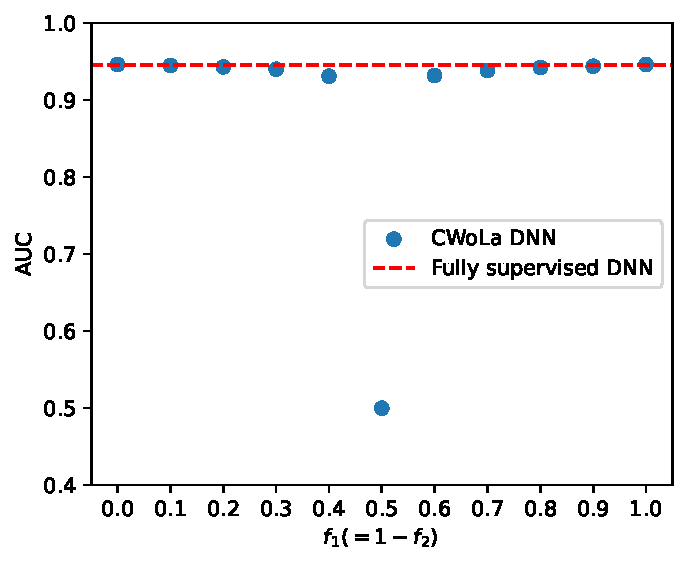
\includegraphics[width=0.45\textwidth]{CWoLa_DNN.pdf}
			}
			\subfloat[SPANet]{
				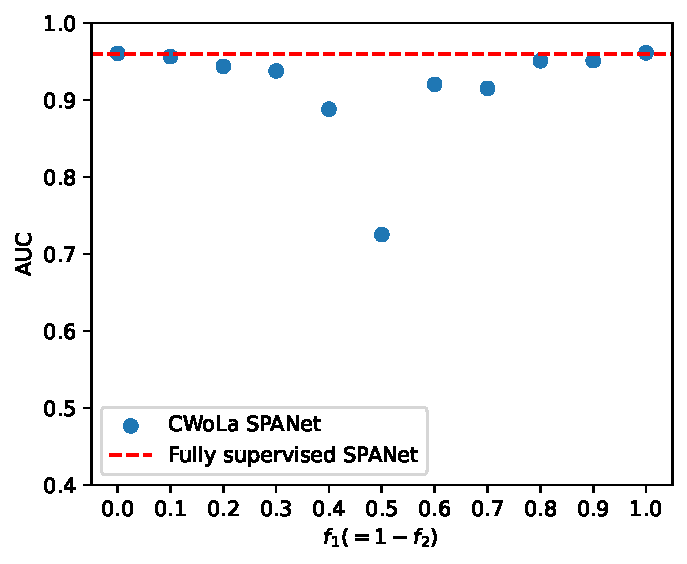
\includegraphics[width=0.45\textwidth]{CWoLa_SPANet.pdf}
			}
			\caption{The AUC of CWoLa training as a function of the signal fraction $f_1$. For simplicity, we set signal fraction $f_2$ equal to $1 - f_1$. The horizontal dashed line indicates the fully-supervised AUC.}
			\label{fig:CWoLa_training_result}
		\end{figure}

		When $f_1 = 0.5$ the mixed sample $M_1$ and $M_2$ have identical distributions, so the classifier can not learn anything in this case. In the case of DNN, the AUC is $0.5$, as expected. However, for SPANet, the AUC is more than $0.7$.

		This is because SPANet is trained on both pairing and classification tasks simultaneously. The pairing part introduces asymmetries between signal and background samples, leading to the AUC that deviates from $0.5$.

		To investigate the effect of the pairing task on SPANet's performance, the weight of the pairing component is set to zero, meaning that SPANet focuses solely on the classification task. Figure~\ref{fig:CWoLa_SPANet_without_pairing} shows the SPANet training results without pairing task. As expected, the AUC is close to $0.5$ when $f_1 = 0.5$. 
		\begin{figure}[htpb]
			\centering
			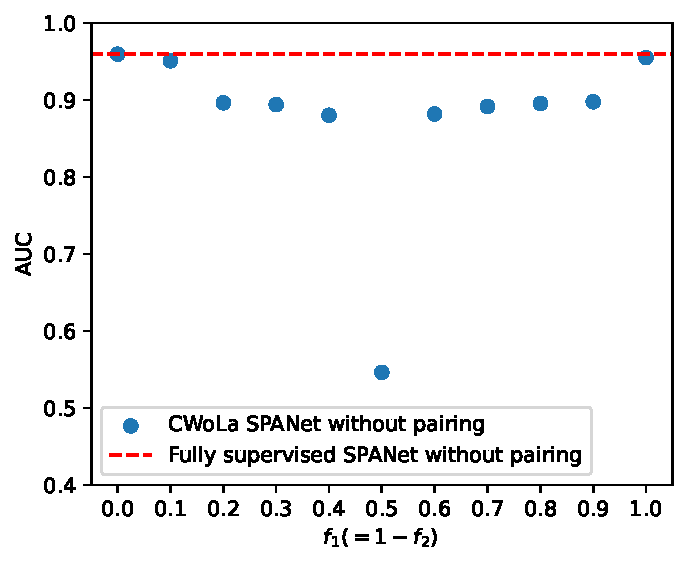
\includegraphics[width=0.65\textwidth]{CWoLa_SPANet_no_pair.pdf}
			\caption{The AUC of CWoLa SPANet training as a function of the signal fraction $f_1$. For simplicity, we set signal fraction $f_2$ equal to $1 - f_1$. Here, SPANet is trained on the classification task only.}
			\label{fig:CWoLa_SPANet_without_pairing}
		\end{figure}	
	% subsection result (end)	
% section cwola (end)

\section{CWoLa hunting}% (fold)
\label{sec:cwola_hunting}
	The CWoLa hunting approach considers a variable $m_{\text{res}}$. For background, the $m_{\text{res}}$ distribution is smooth while signal $m_{\text{res}}$ distribution is expected to be localized near some $m_0$. Consequently, this variable could be used to create two mixed samples. Additional features that are uncorrelated with $m_{\text{res}}$ can be used for training a classifier. This technic is first introduced by Reference~\cite{Collins:2018epr}.
	\subsection{Sample}% (fold)
	\label{sub:sample_cwola_hunting}
		The signal is the resonant Higgs boson pairs production in the four-$b$ quarks channel. In this section, the Higgs boson pair is produced by the heavy CP-even scalar $H$ with mass $m_H = \text{500 GeV}$ or $m_H = \text{1000 GeV}$. The background consists of QCD multi-jet events. The basic requirement is the ``four-tag cut,'' which requires at least four $b$-tagged $R = 0.4$ anti-$k_t$ jets with $p_\text{T} > \text{40 GeV}$ and $\abs{\eta} < 2.5$. Only the events passing the four-tag cut are used in the following analysis.
		
		The CWoLa hunting approach utilizes the signal and sideband regions to create the mixed training sample. The di-Higgs system's total invariant mass $m_{hh}$ is utilized to determine the signal and sideband region. This quantity is computed from the four $b$-jets with the highest transverse momentum. Figure~\ref{fig:mhh_distribution} presents the $m_{hh}$ distribution of signal and background samples. Table~\ref{tab:signal_sideband_range} summarizes the signal and sideband regions. These signal and sideband regions are chosen such that the corresponding cross-sections are closed.
		\begin{figure}[htpb]
			\centering
			\subfloat[$m_H = \text{500 GeV}$]{
				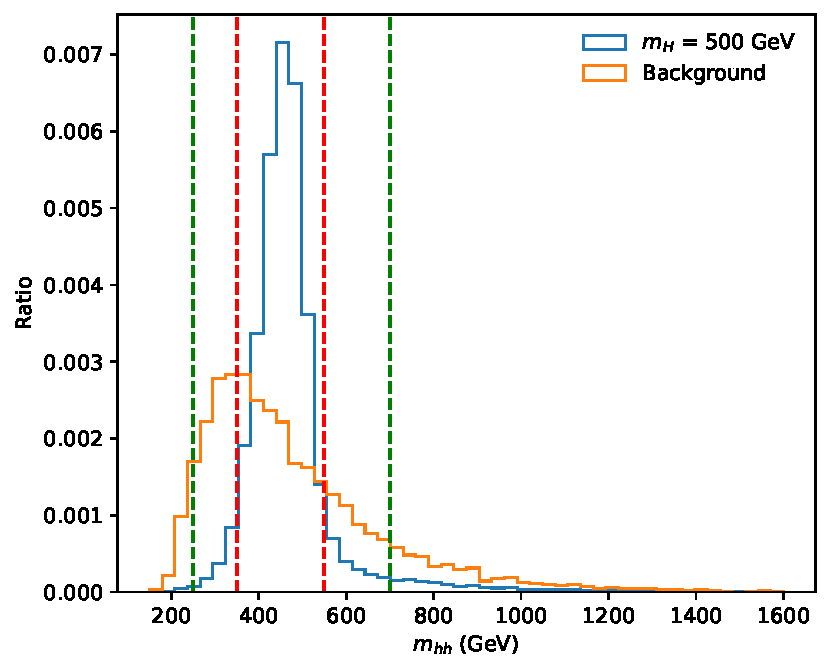
\includegraphics[width=0.45\textwidth]{mhh_distribution-500GeV.pdf}
			}
			\subfloat[$m_H = \text{1000 GeV}$]{
				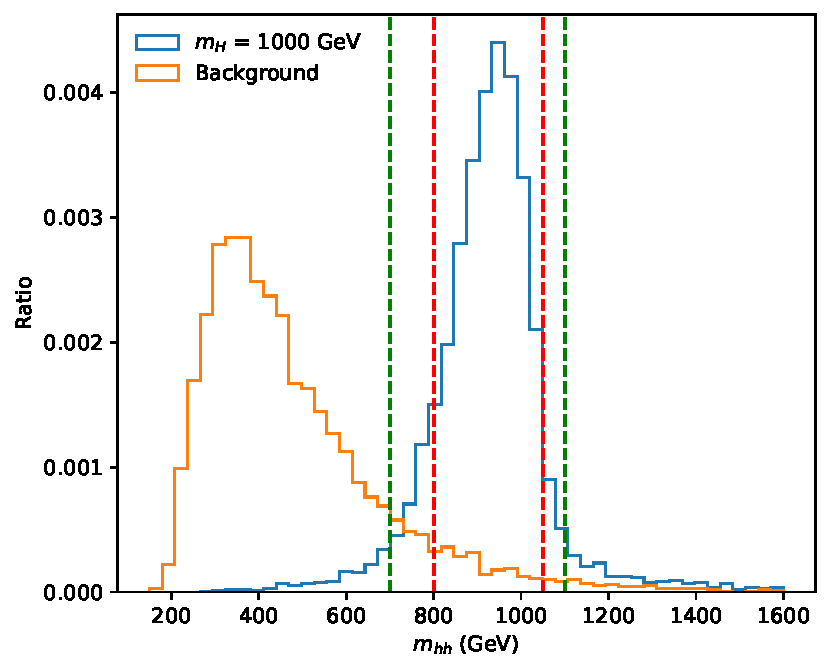
\includegraphics[width=0.45\textwidth]{mhh_distribution-1000GeV.pdf}
			}
			\caption{The total invariant mass $m_{hh}$ distribution of signal and background samples. The signal region is between the red dashed lines. The sideband region is between the green dashed lines and excludes the signal region.}
			\label{fig:mhh_distribution}
		\end{figure}

		\begin{table}[htpb]
			\centering
			\caption{The signal and sideband regions with different resonant samples. The unit is GeV.}
			\label{tab:signal_sideband_range}
			\begin{tabular}{r|cc}
				$m_H$ & Signal       & Sideband                      \\ \hline
				500   & $[350, 550]$ & $[250, 350]\cup [550, 700]$   \\
				1000  & $[800,1050]$ & $[700, 800]\cup [1050, 1100]$
			\end{tabular}
		\end{table}
		Table~\ref{tab:diHiggs_cutflow_table} is the cutflow table of the selection cuts. The number of events used in mixed training samples could be computed from these cross-sections. The training sample size is presented in Table~\ref{tab:training_sample_size_cwola_hunting}.
		\begin{table}[htpb]
			\centering
			\caption{The cross sections for the di-Higgs signal and background processes at different selection cuts.}
			\label{tab:diHiggs_cutflow_table}
			\begin{tabular}{c|l|cc|c|c}
									  &                 & \multicolumn{2}{c|}{Cross section (fb)} &          & $\mathcal{L} = 139 \text{ fb}^{-1}$ \\
				$m_H$ (GeV)           &                 & Signal           & Background           & $S / B$  & $S/\sqrt{B}$                        \\ \hline 
				\multirow{3}{*}{500}  & Four tag        & 3.64             & 6.03e+03             & 6.03e-04 & 0.553                               \\ \cline{2-6} 
									  & Signal region   & 3.13             & 2.57e+03             & 1.22e-03 & 0.727                               \\
									  & Sideband region & 0.35             & 2.36e+03             & 1.50e-04 & 0.086                               \\ \hline \hline
				\multirow{3}{*}{1000} & Four tag        & 0.081            & 6.03e+03             & 1.34e-05 & 0.0123                              \\ \cline{2-6} 
									  & Signal region   & 0.063            & 3.32e+02             & 1.90e-04 & 0.0408                              \\
									  & Sideband region & 0.010            & 3.19e+02             & 3.03e-05 & 0.0064                             
			\end{tabular}
		\end{table}
		
		\begin{table}[htpb]
			\centering
			\caption{The training sample size for the mixed sample. The luminosity is $\mathcal{L} = 78 \text{ fb}^{-1}$ because the generated samples are not enough for now.}
			\label{tab:training_sample_size_cwola_hunting}
			\begin{tabular}{c|c|cc}
									  &              & \multicolumn{2}{c}{True label} \\
				$m_H$ (GeV)           & Mixed sample & Signal       & Background      \\ \hline
				\multirow{2}{*}{500}  & $M_1$        & 244          & 200k            \\
									  & $M_2$        & 28           & 184k            \\ \hline
				\multirow{2}{*}{1000} & $M_1$        & 5            & 26k             \\
									  & $M_2$        & 1            & 25k            
			\end{tabular}
		\end{table}

		Consider the DNN CWoLa classifier. The Higgs candidates are reconstructed by the $\text{min-}\Delta R$ pairing method. In the $\text{min-}\Delta R$ method, the four $b$-tagged jets with the highest $p_{\text{T}}$ are used to form the two Higgs boson candidates. The $\text{min-}\Delta R$ method selects the pairing configuration in which the higher-$p_{\text{T}}$ jet pair has the smallest $\Delta R$ separation. The input features are similar to the previous case (Table~\ref{tab:DNN_variables}), but the $b$-tagging information and the di-Higgs system's total invariant mass are excluded. For $\text{min-}\Delta R$ pairing, it only uses the $b$-tagged jets. Total invariant mass is already used to determine the signal and sideband region.

	% subsection sample_cwola_hunting (end)
	\subsection{Training results}% (fold)
	\label{sub:training_results}
		Table \ref{tab:cwola_hunting_DNN_results} presents the DNN classification training results. These numbers are evaluated from the pure samples, which consist of 5k signal events and 5k background events. The training datasets with and without signal events have similar results. This suggests that the DNN fails to distinguish the signal and background samples but learns the difference between the signal and sideband region. Moreover, the results also imply the input features may correlate to the total invariant mass of the di-Higgs system.
		\begin{table}[htpb]
			\centering
			\caption{The CWoLa DNN training results. ACC is the best accuracy and AUC is the area under the ROC curve. The average and standard deviation of 10 training are presented.}
			\label{tab:cwola_hunting_DNN_results}
			\begin{tabular}{c|c|cc}
				$m_H$ (GeV)           &             & ACC               & AUC               \\ \hline
				\multirow{2}{*}{500}  & With signal & $0.708 \pm 0.002$ & $0.770 \pm 0.007$ \\
									  & No signal   & $0.705 \pm 0.003$ & $0.769 \pm 0.009$ \\ \hline
				\multirow{2}{*}{1000} & With signal & $0.868 \pm 0.024$ & $0.925 \pm 0.023$ \\
									  & No signal   & $0.850 \pm 0.033$ & $0.909 \pm 0.026$
			\end{tabular}
		\end{table}

		Figure~\ref{fig:signal_score_distribution} shows the signal score distributions. Even though the signal scores are very different for signal and background distributions, the difference probably stems from the $m_{hh}$ distribution.
	 	\begin{figure}[htpb]
			\centering
			\subfloat[$m_H = \text{500 GeV}$]{
				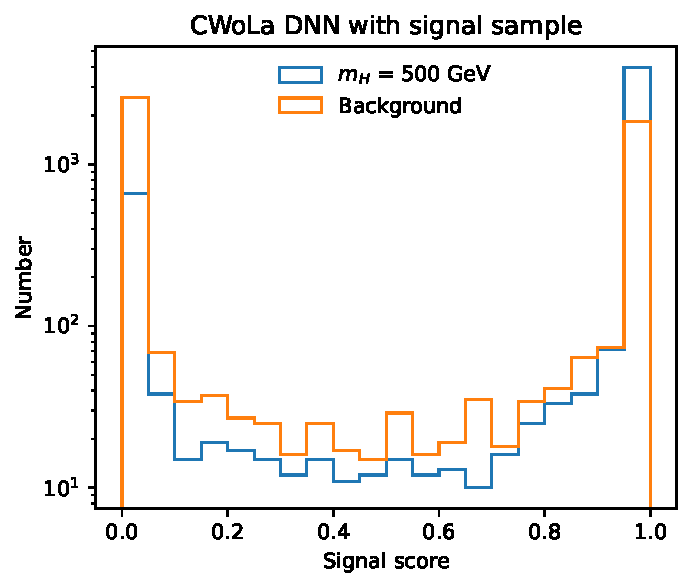
\includegraphics[width=0.45\textwidth]{DNN_w_sig_signal_score_distribution-500GeV.pdf}
				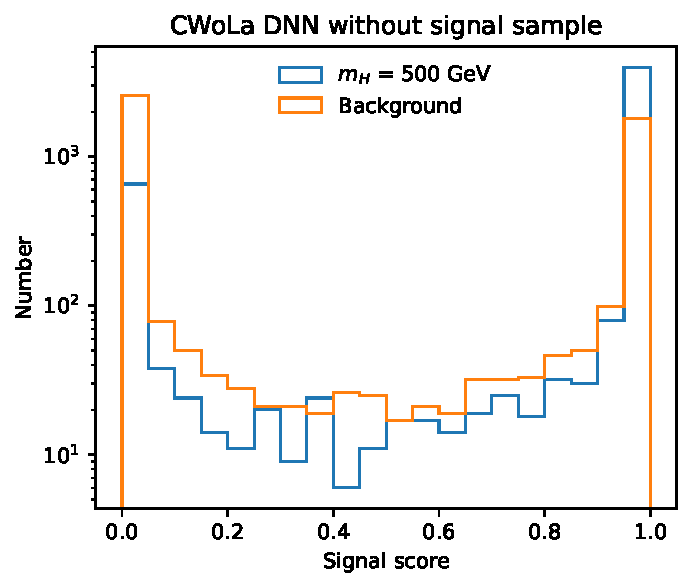
\includegraphics[width=0.45\textwidth]{DNN_wo_sig_signal_score_distribution-500GeV.pdf}
			}
			\\
			\subfloat[$m_H = \text{1000 GeV}$]{
				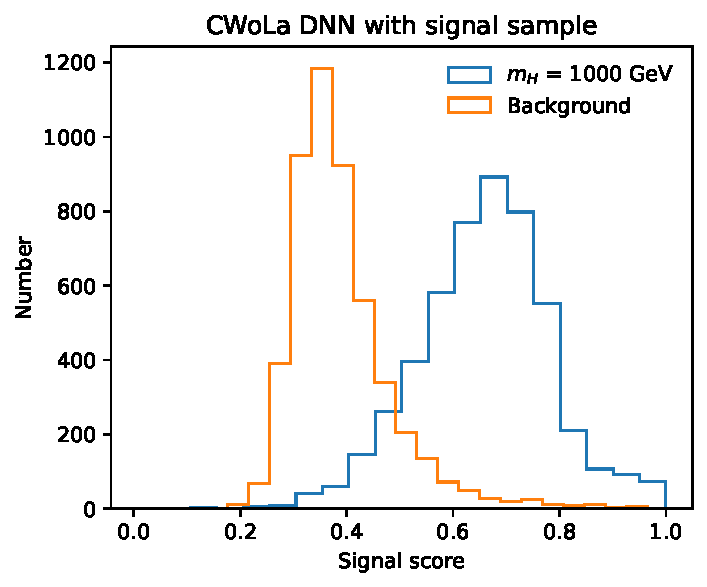
\includegraphics[width=0.45\textwidth]{DNN_w_sig_signal_score_distribution-1000GeV.pdf}
				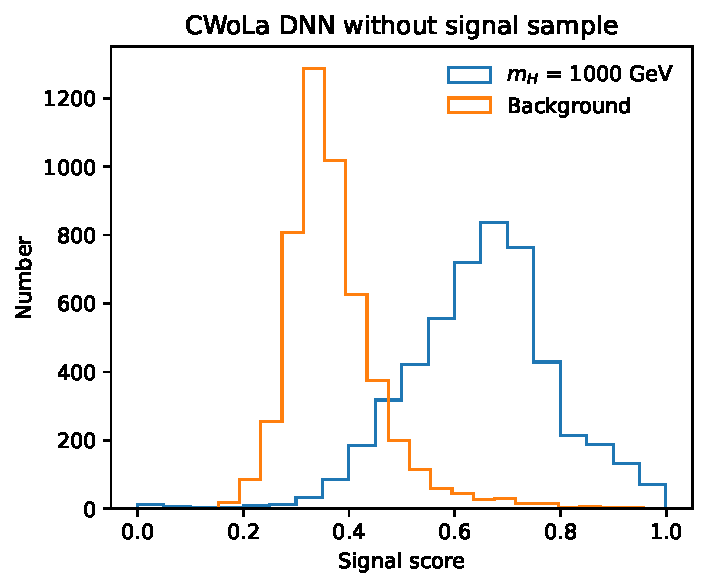
\includegraphics[width=0.45\textwidth]{DNN_wo_sig_signal_score_distribution-1000GeV.pdf}
			}
			\caption{The signal score distributions. We apply the CWoLa DNN on pure samples to obtain the signal score distributions.}
			\label{fig:signal_score_distribution}
		\end{figure}

		There are two issues:
		\begin{itemize}
			\item The input features might correlated to the observables used to determine the signal and sideband region. We need to construct other independent input variables.
			\item The signal fraction is too low. It is hard to learn something about signal events. 
		\end{itemize}
	% subsection training_results (end)
	\subsection{Correlation matrix}% (fold)
	\label{sub:correlation_matrix}
		The results in Section~\ref{sub:training_results} imply that the di-Higgs system's total invariant mass is not independent of other input features. To find the variables that are highly dependent on the total invariant mass, the correlation coefficients are computed among these variables. Figure~\ref{fig:correlation_coefficient_500GeV} and \ref{fig:correlation_coefficient_1000GeV} are correlation coefficients on the $\text{500 GeV}$ and $\text{1000 GeV}$ cases, respectively. 

		\begin{figure}[htpb]
			\centering
			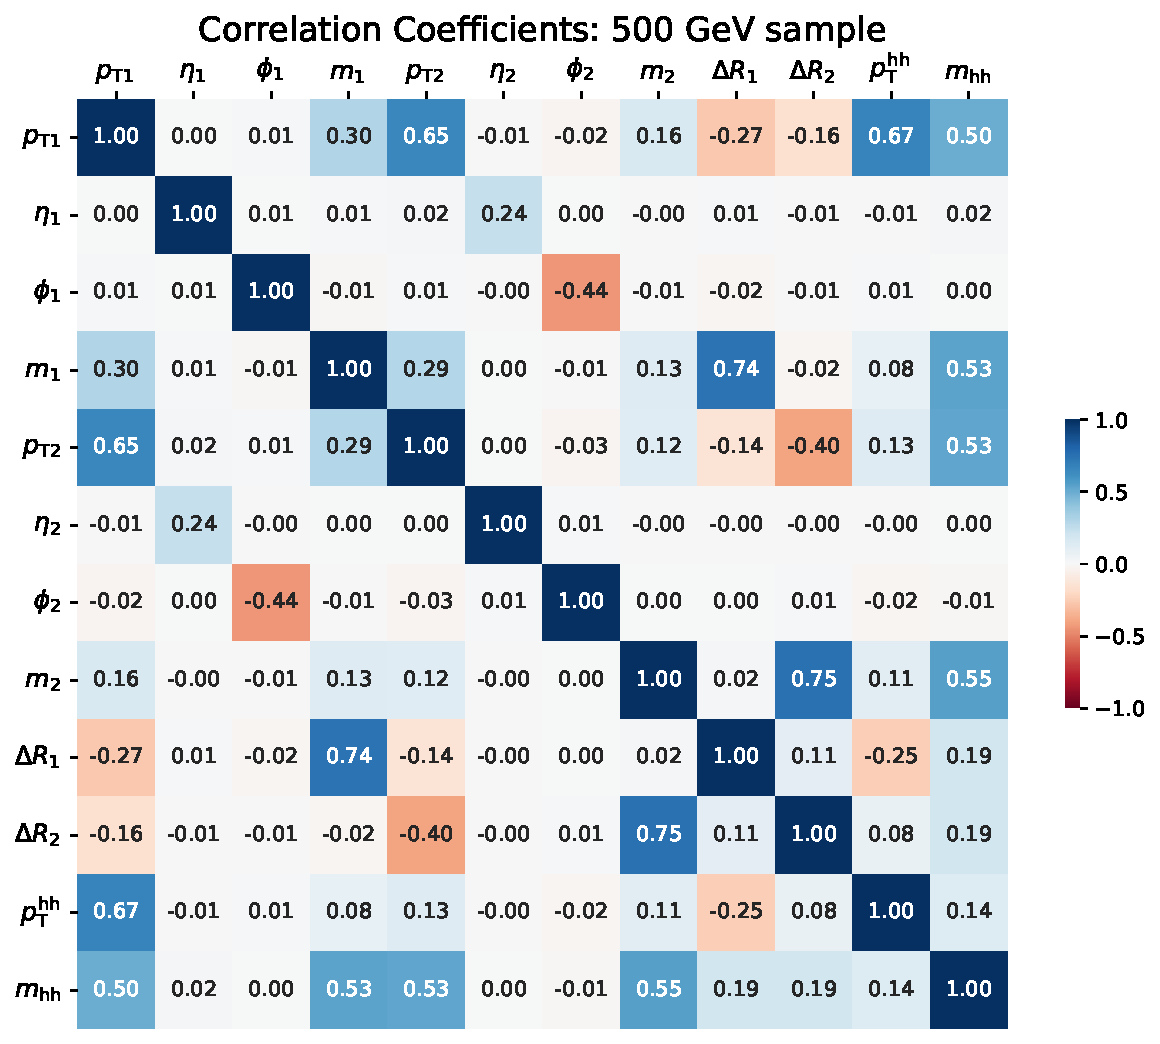
\includegraphics[width=0.9\textwidth]{correlation_coefficients-500GeV.pdf}
			\caption{The correlation coefficients among different variables, which are computed from $\text{500 GeV}$ testing sample, which consists of 5k signal and 5k background.}
			\label{fig:correlation_coefficient_500GeV}
		\end{figure}
		
		\begin{figure}[htpb]
			\centering
			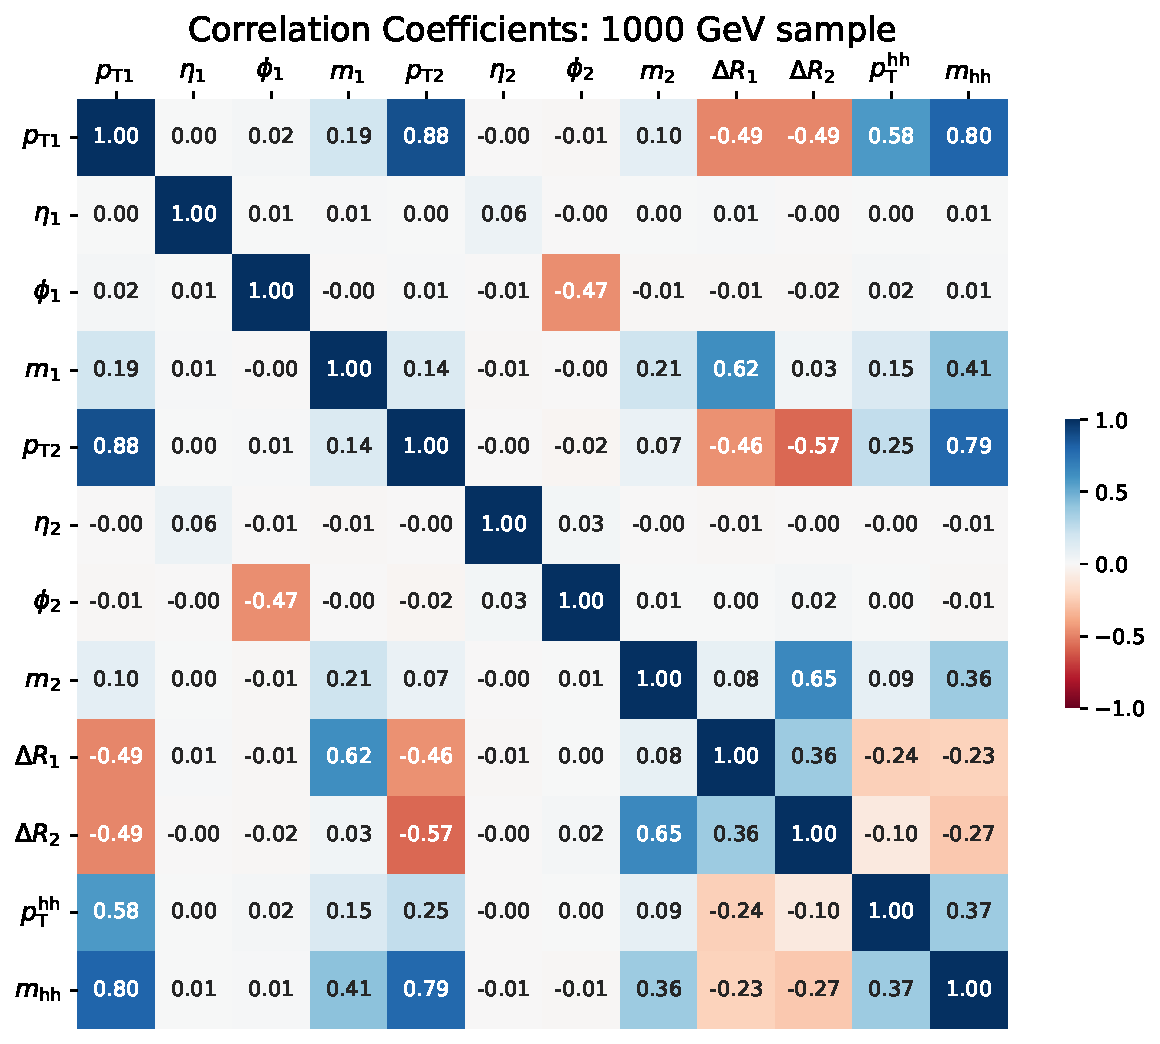
\includegraphics[width=0.9\textwidth]{correlation_coefficients-1000GeV.pdf}
			\caption{The correlation coefficients among different variables, which are computed from $\text{1000 GeV}$ testing sample, which consists of 5k signal and 5k background.}
			\label{fig:correlation_coefficient_1000GeV}
		\end{figure}

		The results show that the transverse momentum $p_\text{T}$ and the invariant mass $m$ of Higgs candidates are highly correlated to the total invariant mass. Figure~\ref{fig:pt1_mhh_scatter_plot} shows the scatter plots of the transverse momentum of the leading Higgs candidate and the total invariant mass $m_{\text{hh}}$. These plots also explain why the DNN only trained on background samples can distinguish the signal and background events, because the background distribution in the signal and sideband regions are different.  
		\begin{figure}[htpb]
			\centering
			\subfloat[$m_H = \text{500 GeV}$]{
				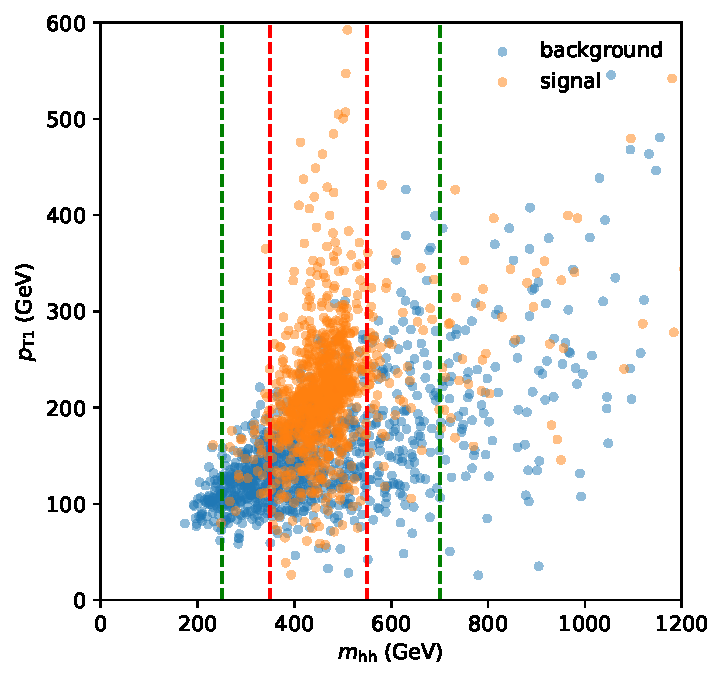
\includegraphics[width=0.45\textwidth]{scatter_plot_mhh_pt1-500GeV.pdf}
			}
			\subfloat[$m_H = \text{1000 GeV}$]{
				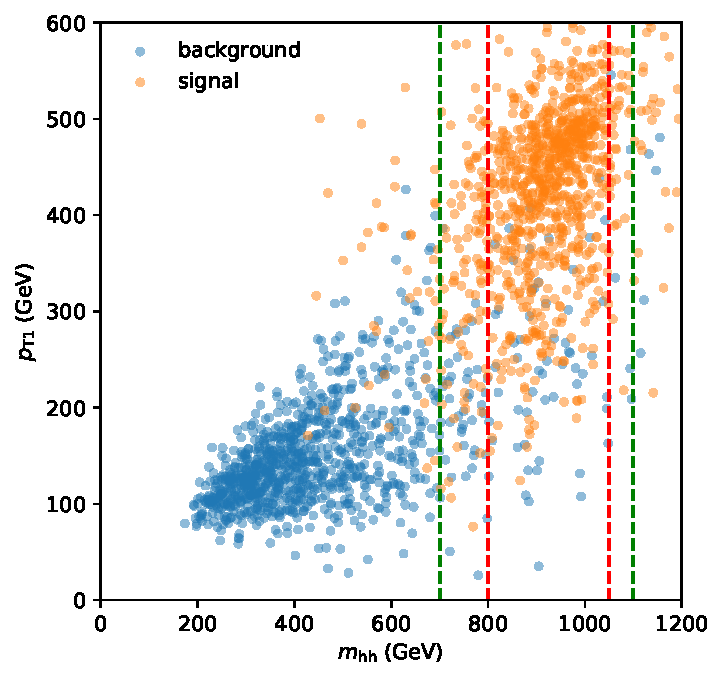
\includegraphics[width=0.45\textwidth]{scatter_plot_mhh_pt1-1000GeV.pdf}
			}
			\caption{The scatter plots of the transverse momentum of leading Higgs candidate $p_{\text{T}1}$ and total invariant mass $m_{hh}$ distribution. The signal region is between the red dashed lines. The sideband region is between the green dashed lines and excludes the signal region.}
			\label{fig:pt1_mhh_scatter_plot}
		\end{figure}
	% subsection correlation_matrix (end)
	\subsection{Remove highly correlated features}% (fold)
	\label{sub:remove_highly_correlated_features}
		 Figure~\ref{fig:correlation_coefficient_500GeV} and \ref{fig:correlation_coefficient_1000GeV} show that the transverse momentum $p_\text{T}$ and the invariant mass $m$ of Higgs candidates are highly related to the total invariant mass $m_{hh}$. To investigate the impact of these highly correlated features on the discrimination power of CWoLa DNN models, we remove these input features and train the DNN model again.

		\begin{table}[htpb]
			\centering
			\caption{The CWoLa DNN training results. The transverse momentum and invariant mass of Higgs candidates are removed from samples. ACC is the best accuracy and AUC is the area under the ROC curve. The average and standard deviation of 10 training are presented.}
			\label{tab:cwola_hunting_DNN_results_wo_pt_m}
			\begin{tabular}{c|c|cc}
				$m_H$ (GeV)           &             & ACC               & AUC               \\ \hline
				\multirow{2}{*}{500}  & With signal & $0.526 \pm 0.020$ & $0.536 \pm 0.053$ \\
									  & No signal   & $0.532 \pm 0.015$ & $0.543 \pm 0.029$ \\ \hline
				\multirow{2}{*}{1000} & With signal & $0.586 \pm 0.030$ & $0.625 \pm 0.046$ \\
									  & No signal   & $0.564 \pm 0.024$ & $0.583 \pm 0.042$
			\end{tabular}
		\end{table}

		 Table~\ref{tab:cwola_hunting_DNN_results_wo_pt_m} summarizes the results of the CWoLa DNN training without $p_{\text{T}}$ and $m$ features. The training datasets with and without signal events still have similar results. Compared to the previous one (Table~\ref{tab:cwola_hunting_DNN_results}) the accuracy values are closer to 0.5. These results suggest that the removed features have a significant contribution to the model's discrimination power, and the remaining parameters are hard to utilize to distinguish the signal and background events.
	% subsection remove_highly_correlated_features (end)	
	\subsection{Transverse momentum cut testing}% (fold)
	\label{sub:pt_cut_testing}
		In Figure~\ref{fig:mhh_distribution}, the distribution of the background sample exhibits a gradual termination around $\text{150 GeV}$. To investigate whether this termination is a result of the ``four-tag cut'', which requires $p_{\text{T}} > \text{40 GeV}$, total invariant mass distributions with different $p_{\text{T}}$ cuts are plotted in Figure~\ref{fig:mhh_distribution_bkg_pt}. As the transverse momentum requirement increases from $\text{40 GeV}$ to $\text{70 GeV}$, the termination point also shifts to larger values. Moreover, the termination remains gradual rather than an abrupt cut-off, suggesting that the gradual termination indeed results from the transverse momentum cut.
		\begin{figure}[htpb]
			\centering
			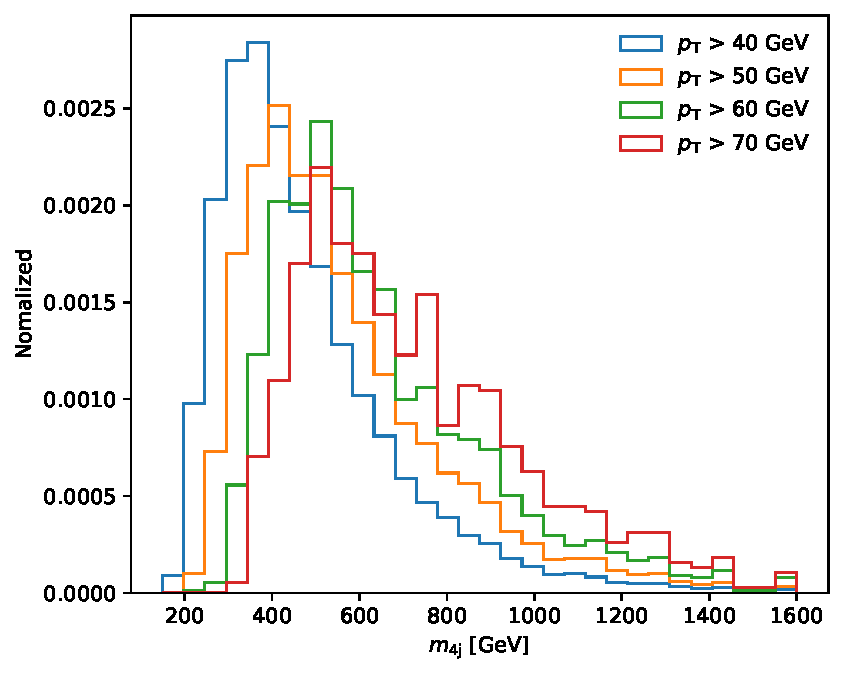
\includegraphics[width=0.5\textwidth]{m4j_distribution_background_various_pt_cut.pdf}
			\caption{The total invariant mass $m_{\text{4j}}$ distribution of background samples. The transverse momentum requirement is varied from $\text{40 GeV}$ to $\text{70 GeV}$.}
			\label{fig:mhh_distribution_bkg_pt}
		\end{figure}
	% subsection pt_cut_testing (end)
	\subsection{Enlarge the signal sample size}% (fold)
	\label{sub:enlarge_the_signal_sample_size}
		Another issue arises from the low signal fraction (Table~\ref{tab:training_sample_size_cwola_hunting}), making DNN difficult to extract meaningful information about signal events. To investigate the impact of signal sample size, we increase the signal size manually and retrain the DNN model. The training sample sizes are summarized in Table~\ref{tab:training_sample_size_cwola_hunting_enlarge_signal_size}.

		\begin{table}[htpb]
			\centering
			\caption{The training sample size for the mixed sample. Various signal sizes are considered, and the background sizes are fixed for all cases. ``1 times'' represents the previous ``With signal'' case and ``0 times'' represents the previous ``No signal'' case.}
			\label{tab:training_sample_size_cwola_hunting_enlarge_signal_size}
			\begin{tabular}{c|c|cccc|c}
									  &              & \multicolumn{4}{c|}{Signal}              & Background \\ \hline
				$m_H$ (GeV)           & Mixed sample & 1 times & 0 times & 10 times & 100 times & All        \\ \hline
				\multirow{2}{*}{500}  & $M_1$        & 244     & 0       & 2438     & 24380     & 200k       \\
									  & $M_2$        & 28      & 0       & 276      & 2760      & 184k       \\ \hline
				\multirow{2}{*}{1000} & $M_1$        & 5       & 0       & 49       & 492       & 26k        \\
									  & $M_2$        & 1       & 0       & 8        & 75        & 25k       
			\end{tabular}
		\end{table}

		\begin{table}[htpb]
			\centering
			\caption{The CWoLa DNN training results. The transverse momentum and invariant mass of Higgs candidates are removed from samples. 1 time and 0 times are the with signal and no signal case in Table~\ref{tab:cwola_hunting_DNN_results_wo_pt_m}. ACC is the best accuracy and AUC is the area under the ROC curve. The average and standard deviation of 10 training are presented.}
			\label{tab:cwola_hunting_DNN_results_wo_pt_m_enlarge_signal_size}
			\begin{tabular}{c|c|cc}
				$m_H$ (GeV)           & times & ACC               & AUC               \\ \hline
				\multirow{4}{*}{500}  & 1     & $0.526 \pm 0.020$ & $0.536 \pm 0.053$ \\
									  & 10    & $0.531 \pm 0.027$ & $0.533 \pm 0.045$ \\
									  & 100   & $0.634 \pm 0.014$ & $0.751 \pm 0.030$ \\
									  & 0     & $0.532 \pm 0.015$ & $0.543 \pm 0.029$ \\ \hline
				\multirow{4}{*}{1000} & 1     & $0.586 \pm 0.030$ & $0.625 \pm 0.046$ \\
									  & 10    & $0.626 \pm 0.027$ & $0.678 \pm 0.040$ \\
									  & 100   & $0.621 \pm 0.012$ & $0.670 \pm 0.023$ \\
									  & 0     & $0.564 \pm 0.024$ & $0.583 \pm 0.042$
			\end{tabular}
		\end{table}

		Table~\ref{tab:cwola_hunting_DNN_results_wo_pt_m_enlarge_signal_size} provides the results of the CWoLa DNN training without $p_{\text{T}}$ and $m$ features. For the $\text{500 GeV}$ case, the ``0 times,'', ``1 times,'' and ``10 times'' samples yield similar results, while ``100 times'' sample exhibits better performance. This suggests that the CWoLa DNN can extract meaningful information from the ``100 times'' sample. In the case of $\text{1000 GeV}$, we can obtain better results when the signal sample size increases. The performance of 10 times and 100 times is similar. It seems that the training performance is saturated. 

		To further understand the behavior between 10 times and 100 times samples for the $\text{500 GeV}$ case, additional samples within this size range are generated, and the DNN is trained on these samples.

		\begin{figure}[htpb]
			\centering
			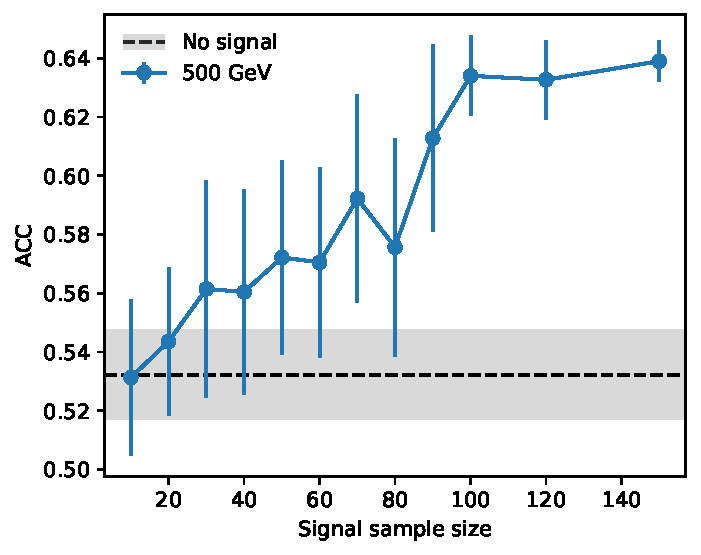
\includegraphics[width=0.55\textwidth]{ACC_vs_signal_sample_size-500GeV.pdf}
			\caption{The accuracy of CWoLa DNN training as a function of the signal size. The unit of sample size is the size of the ``1 times'' case. The error bar is the standard deviation of 10 training. The grey band is the error bar of the ``without signal'' case.}
			\label{fig:cwola_hunting_DNN_results_wo_pt_m_various_signal_size_500GeV}
		\end{figure}

		Figure~\ref{fig:cwola_hunting_DNN_results_wo_pt_m_various_signal_size_500GeV} is the training performance against the signal sample size. In this region, the performance increases when the signal size is increased. 120 times and 150 times samples are also generated and used in training. The accuracy is saturated at around 63\%.

		Similarly, for the $\text{1000 GeV}$ case, the DNN is trained on samples with sizes ranging from 1 to 10 times. Figure~\ref{fig:cwola_hunting_DNN_results_wo_pt_m_various_signal_size_1000GeV} is the training performance against the signal sample size. The performance is similar for all cases. The training accuracy is saturated at around 62\%.
		\begin{figure}[htpb]
			\centering
			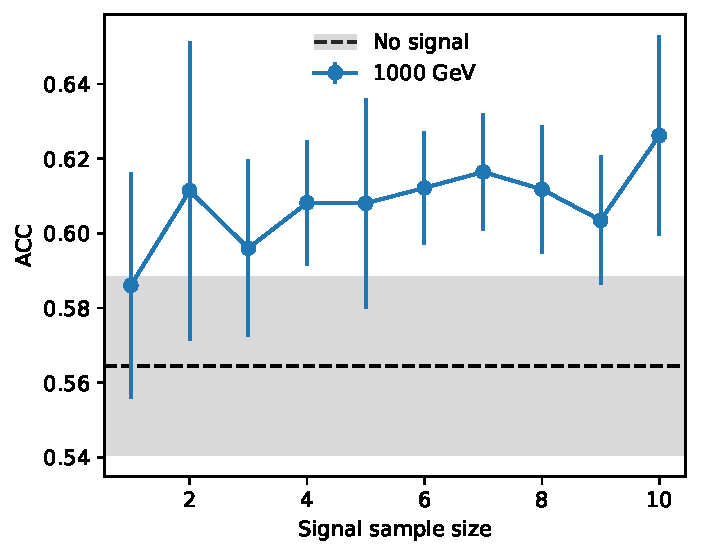
\includegraphics[width=0.55\textwidth]{ACC_vs_signal_sample_size-1000GeV.pdf}
			\caption{The performance of CWoLa DNN training as a function of the signal size. The unit of sample size is the size of the ``1 times'' case. The error bar is the standard deviation of 10 times training. The grey band is the error bar of the ``without signal'' case.}
			\label{fig:cwola_hunting_DNN_results_wo_pt_m_various_signal_size_1000GeV}
		\end{figure}

	% subsection enlarge_the_signal_sample_size (end)
	\subsection{Training with deeper model}% (fold)
	\label{sub:training_with_deeper_model}
		In Figure~\ref{fig:cwola_hunting_DNN_results_wo_pt_m_various_signal_size_1000GeV}, the performance of CWoLa DNN is quickly saturated. To investigate the impact of the model structure, the deeper DNN model is trained. In Section~\ref{sub:enlarge_the_signal_sample_size}, DNN consists of 2 hidden layers, while in this section we train the DNN with 4 hidden layers.

		The DNN is trained on signal sample size ranging from 1 to 500 times. Table~\ref{tab:cwola_hunting_DNN_results_wo_pt_m_enlarge_signal_size_deeper_model} and Figure~\ref{fig:cwola_hunting_DNN_results_wo_pt_m_various_signal_size_deeper_model_1000GeV} are the training results. The performance is generally better than the previous results (Table~\ref{tab:cwola_hunting_DNN_results_wo_pt_m_enlarge_signal_size}), even for the without signal case. It seems that the previous model structure is too simple and it limits the training performance. For the signal size within 1 times to 300 times, the performance increases when the signal size is increased. After this region, the accuracy does not significantly improve. The accuracy is saturated at around 67\%, but this value is still better than the previous ones.

		\begin{table}[htpb]
			\centering
			\caption{The CWoLa DNN training results. The transverse momentum and invariant mass of Higgs candidates are removed from samples. 1 time and 0 times are the with signal and no signal case in Table~\ref{tab:cwola_hunting_DNN_results_wo_pt_m}. ACC is the best accuracy and AUC is the area under the ROC curve. The average and standard deviation of 10 training are presented.}
			\label{tab:cwola_hunting_DNN_results_wo_pt_m_enlarge_signal_size_deeper_model}
			\begin{tabular}{c|c|cc}
				$m_H$ (GeV)           & times & ACC               & AUC               \\ \hline
				\multirow{4}{*}{1000} & 1     & $0.613 \pm 0.017$ & $0.649 \pm 0.021$ \\
									  & 10    & $0.622 \pm 0.018$ & $0.673 \pm 0.033$ \\
									  & 100   & $0.639 \pm 0.022$ & $0.695 \pm 0.034$ \\
									  & 0     & $0.602 \pm 0.022$ & $0.643 \pm 0.042$
			\end{tabular}
		\end{table}
		\begin{figure}[htpb]
			\centering
			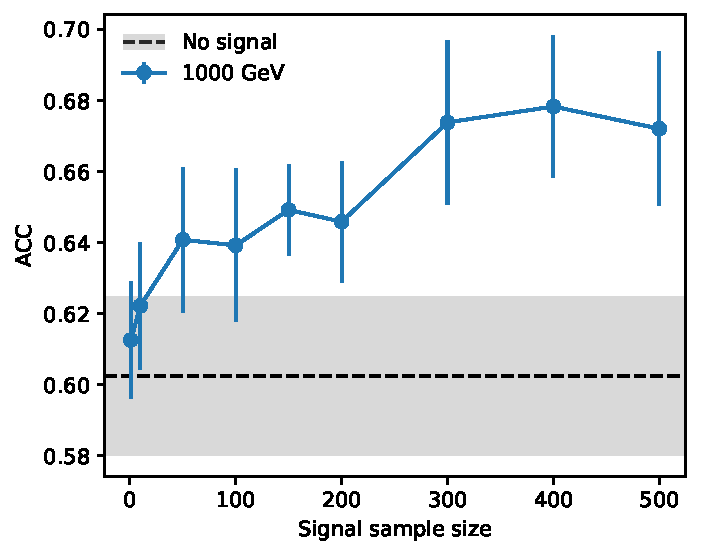
\includegraphics[width=0.55\textwidth]{ACC_vs_signal_sample_size_deeper_model-1000GeV.pdf}
			\caption{The performance of CWoLa DNN training as a function of the signal size. The unit of sample size is the size of the ``1 times'' case. The error bar is the standard deviation of 10 times training. The grey band is the error bar of the ``without signal'' case.}
			\label{fig:cwola_hunting_DNN_results_wo_pt_m_various_signal_size_deeper_model_1000GeV}
		\end{figure}
	% subsection training_with_deeper_model (end)	
% section cwola_hunting (end)		
\section{Physical data augmentation}% (fold)
\label{sec:physical_data_augmentation}
	The physical augmentations are inspired by Reference~\cite{Dillon:2023zac}, which considers the rotation and smearing augmentations. These augmentations reflect both the symmetries in the physical event and the experimental resolution of the detector.
	\subsection{Original training data}% (fold)
	\label{sub:original_training_data}
		The signal is the resonant Higgs boson pairs production in the four-$b$ quarks channel. In this section, the Higgs boson pair is produced by the heavy CP-even scalar $H$ with mass $m_H = \text{500 GeV}$. The background consists of QCD multi-jet events. The basic requirement is the ``four-tag cut,'' which requires at least four $b$-tagged $R = 0.4$ anti-$k_t$ jets with $p_\text{T} > \text{40 GeV}$ and $\abs{\eta} < 2.5$. Only the events passing the four-tag cut are used in the following analysis.
		
		The training samples consist of 50k signal events and 50k background events and the testing samples consist of 5k signal events and 5k background events.

		The Higgs candidates are reconstructed by the $\text{min-}\Delta R$ pairing method. The input features are similar to the previous case (Table~\ref{tab:DNN_variables}), but the $b$-tagging information is excluded.
	% subsection original_training_data (end)
	\subsection{Physical augmentation}% (fold)
	\label{sub:physical_augmentation}
		We consider three different physical augmentations.

		\begin{enumerate}
			\item Azimuthal rotation: The final state is rotated by an angle $\phi$ randomly sampled from $[0, 2\pi]$.
			\item $\eta-\phi$ smearing: The $\left( \eta,\phi \right) $ coordinate of Higgs candidates are resampled according to a Normal distribution centered on the original coordinate and with a standard deviation inversely proportional to the $p_{\text{T}}$
				\begin{equation}
					\eta' \sim \mathcal{N}\left(\eta, \frac{\Lambda}{p_{\text{T}}}\right), \quad \phi' \sim \mathcal{N}\left(\phi, \frac{\Lambda}{p_{\text{T}}}\right)
				\end{equation}
				where $\eta', \phi'$ are the augmented coordinate, $p_{\text{T}}$ is the transverse momentum of the Higgs candidate, and the smearing scale is set to be $\Lambda = \text{10 GeV}$.
			\item $p_\text{T}$ smearing: The $p_{\text{T}}$ of Higgs candidates are resampled according to
				\begin{equation}
					p_{\text{T}}' \sim \mathcal{N}\left( p_{\text{T}}, f(p_{\text{T}}) \right), \quad f(p_{\text{T}}) = \sqrt{0.052 p_{\text{T}}^2 + 1.502p_{\text{T}}}
				\end{equation}
				where $p_{\text{T}}'$ is the augmented transverse momentum, $f\left( p_\text{T} \right) $ is the energy smearing applied by \verb|Delphes| (the $p_{\text{T}}$'s are normalised by $\text{1 GeV}$).
		\end{enumerate}

		Figure~\ref{fig:eta_phi_smearing_eta_distribution}, \ref{fig:eta_phi_smearing_phi_distribution} and \ref{fig:pt_smearing_pt_distribution} are the distributions before and after the augmentation. The distributions for the $\eta-\phi$ smearing are similar for both cases. For $p_\text{T}$ smearing, the peak broadens and the transverse momentum distribution looks smoother.
		\begin{figure}[htpb]
			\centering
			\subfloat[Leading Higgs]{
				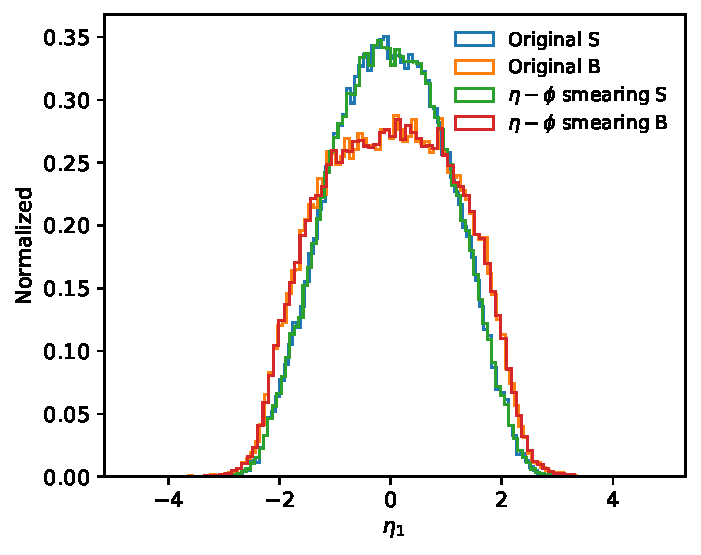
\includegraphics[width=0.45\textwidth]{eta1_distribution_eta_phi_smearing.pdf}
			}
			\subfloat[Sub-leading Higgs]{
				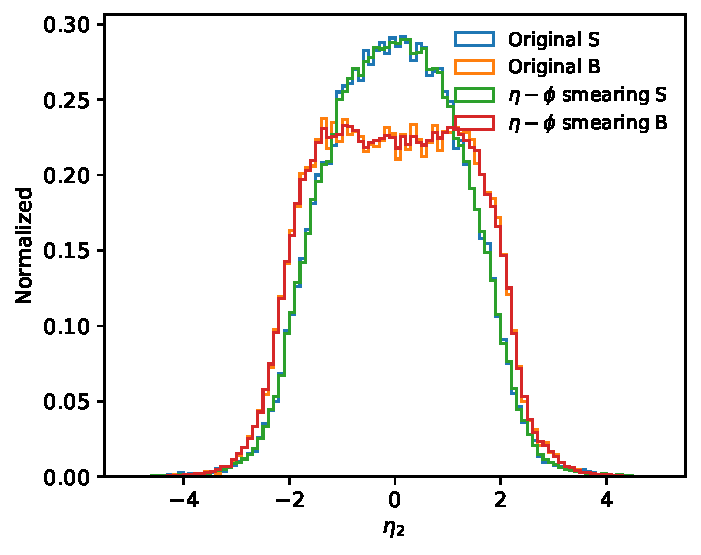
\includegraphics[width=0.45\textwidth]{eta2_distribution_eta_phi_smearing.pdf}
			}
			\caption{The pseudorapidity distribution before and after the $\eta-\phi$ smearing augmentation. $\eta_1$ and $\eta_2$ are the pseudorapidities of the leading and the sub-leading Higgs candidate, respectively.}
			\label{fig:eta_phi_smearing_eta_distribution}
		\end{figure}
		\begin{figure}[htpb]
			\centering
			\subfloat[Leading Higgs]{
				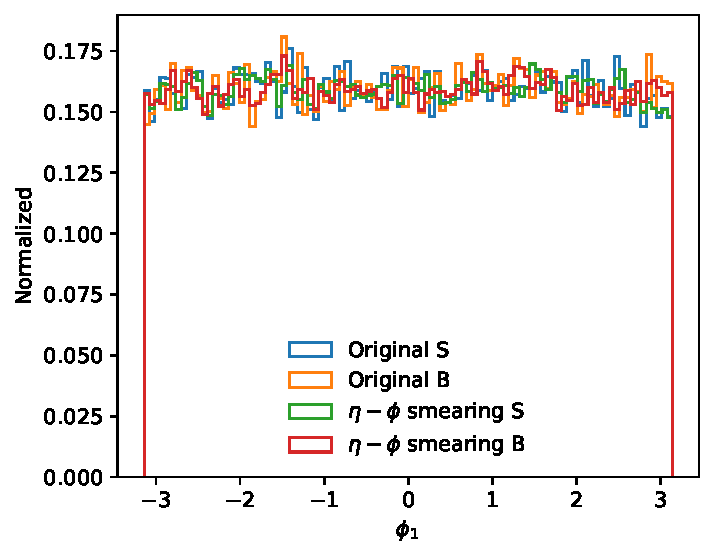
\includegraphics[width=0.45\textwidth]{phi1_distribution_eta_phi_smearing.pdf}
			}
			\subfloat[Sub-leading Higgs]{
				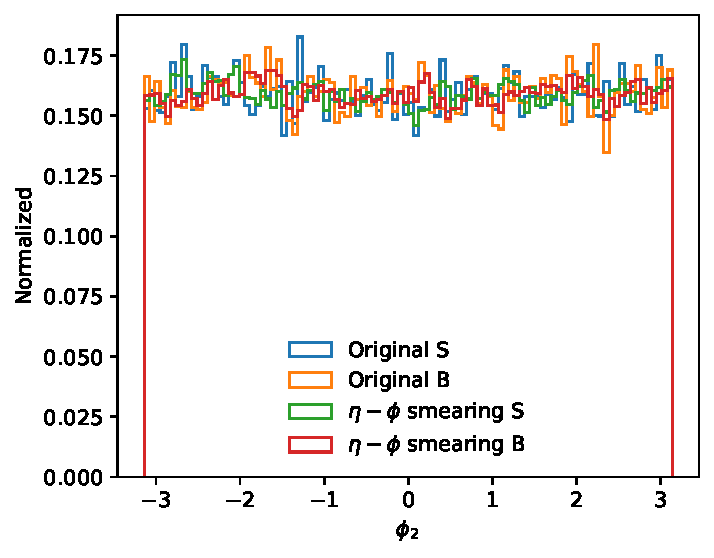
\includegraphics[width=0.45\textwidth]{phi2_distribution_eta_phi_smearing.pdf}
			}
			\caption{The azimuthal angle distribution before and after the $\eta-\phi$ smearing augmentation. $\phi_1$ and $\phi_2$ are the azimuthal angles of the leading and the sub-leading Higgs candidate, respectively.}
			\label{fig:eta_phi_smearing_phi_distribution}
		\end{figure}
		\begin{figure}[htpb]
			\centering
			\subfloat[Leading Higgs]{
				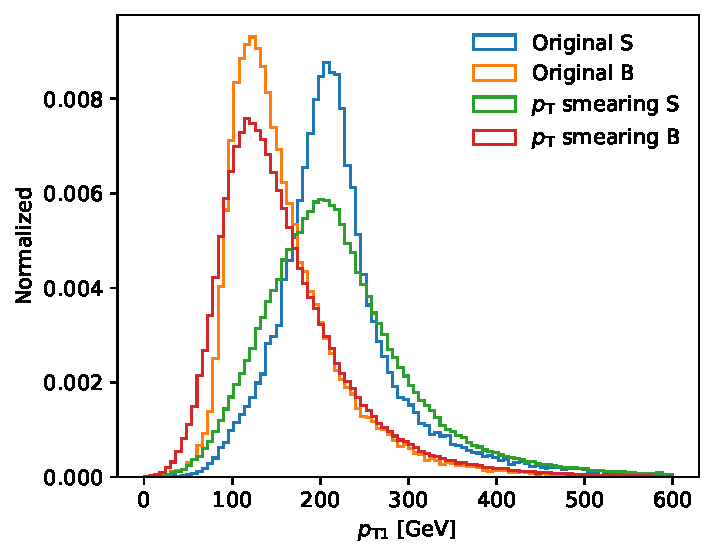
\includegraphics[width=0.45\textwidth]{pt1_distribution_pt_smearing.pdf}
			}
			\subfloat[Sub-leading Higgs]{
				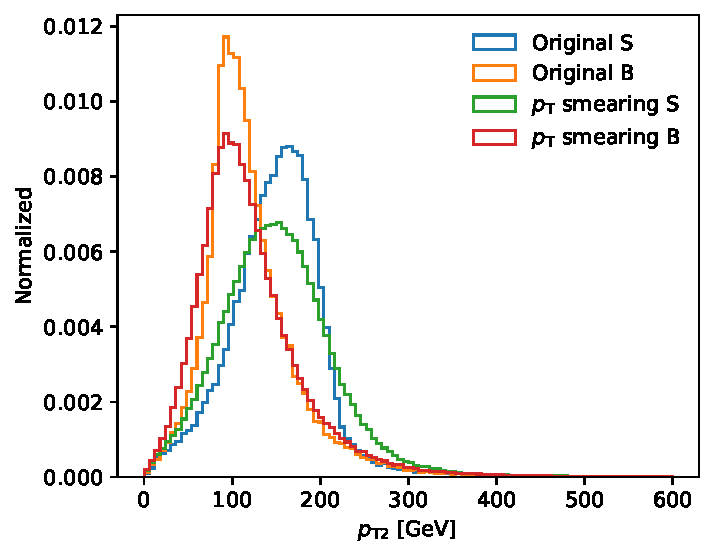
\includegraphics[width=0.45\textwidth]{pt2_distribution_pt_smearing.pdf}
			}
			\caption{The transverse momentum distribution before and after the $p_{\text{T}}$ smearing augmentation. $p_{\text{T1}}$ and $p_{\text{T2}}$ are the transverse momentum of the leading and the sub-leading Higgs candidates, respectively.}
			\label{fig:pt_smearing_pt_distribution}
		\end{figure}

		For each type of augmentation, we test ``$n$ times augmentation'' with different $n$. The $n$ times augmentation means for one original sample, we generate $n$ augmented samples. Additionally, we test another case that applies all augmentations at the same time.
	% subsection physical_augmentation (end)
	\subsection{Training results}% (fold)
	\label{sub:training_results_physical_augmentation}
	
		Table~\ref{tab:original_sample_training_results} presents the DNN classification training results of the original sample. Table~\ref{tab:augmentation_sample_training_results} are the training results of the augmented samples. For each type of augmentation, they all can improve the ACC by about 4\%. The differences among the various augmentation are not significant. The 10-times augmentation has the best results, but the difference between the 5-times and 10-times augmentation is tiny. It seems that the performance of this classifier is saturated.
		\begin{table}[htpb]
			\centering
			\caption{The training results of original samples. ACC is the best accuracy and AUC is the area under the ROC curve. The average and standard deviation of 10 training are presented.}
			\label{tab:original_sample_training_results}
			\begin{tabular}{c|c}
			    & Original \\ \hline
			ACC & $0.845 \pm 0.015$    \\
			AUC & $0.917 \pm 0.005$    
			\end{tabular}
		\end{table}
		\begin{table}[htpb]
			\centering
			\caption{The training results of augmented samples. ``+ 3 times'' means the training sample consists of the original sample and 3 times the augmented sample. ACC is the best accuracy and AUC is the area under the ROC curve. The average and standard deviation of 10 training are presented.}
			\label{tab:augmentation_sample_training_results}
			\begin{tabular}{c|c|cccc}
				Sample                      &     & Rotation          & $\eta-\phi$ smear & $p_{\text{T}}$ smear & All               \\ \hline
				\multirow{2}{*}{+ 3 times}  & ACC & $0.880 \pm 0.007$ & $0.879 \pm 0.010$ & $0.882 \pm 0.003$    & $0.875 \pm 0.011$ \\
											& AUC & $0.950 \pm 0.007$ & $0.949 \pm 0.008$ & $0.951 \pm 0.003$    & $0.942 \pm 0.012$ \\ \hline
				\multirow{2}{*}{+ 5 times}  & ACC & $0.887 \pm 0.002$ & $0.887 \pm 0.001$ & $0.890 \pm 0.002$    & $0.889 \pm 0.003$ \\
											& AUC & $0.955 \pm 0.001$ & $0.955 \pm 0.001$ & $0.957 \pm 0.001$    & $0.956 \pm 0.001$ \\ \hline
				\multirow{2}{*}{+ 10 times} & ACC & $0.889 \pm 0.001$ & $0.889 \pm 0.002$ & $0.892 \pm 0.002$    & $0.892 \pm 0.002$ \\
											& AUC & $0.956 \pm 0.001$ & $0.956 \pm 0.001$ & $0.958 \pm 0.001$    & $0.958 \pm 0.000$
			\end{tabular}
		\end{table}	
		
		
	% subsection training_results_physical_augmentation (end)

	\subsection{Deeper model}% (fold)
	\label{sub:deeper_model}
		In Section~\ref{sub:training_results_physical_augmentation}, the DNN model consists of 2 hidden layers, each containing 64 hidden nodes. To explore the impact of the model structure, the deeper DNN model is trained. We investigate the performance of the DNN model with 5 hidden layers.

		\begin{table}[htpb]
			\centering
			\caption{The training results of deeper DNN model. ``+ 3 times'' means the training sample consists of the original sample and 3 times the augmented sample. ACC is the best accuracy and AUC is the area under the ROC curve. The average and standard deviation of 10 training are presented.}
			\label{tab:augmentation_training_results_deeper_model}
			\begin{tabular}{l|c|cccc}
			Sample                            &     & Original          & + 3 times         & + 5 times         & + 10 times        \\ \hline
			\multirow{2}{*}{All augmentation} & ACC & $0.864 \pm 0.005$ & $0.890 \pm 0.002$ & $0.890 \pm 0.002$ & $0.884 \pm 0.005$ \\
											  & AUC & $0.928 \pm 0.005$ & $0.957 \pm 0.001$ & $0.957 \pm 0.001$ & $0.949 \pm 0.005$
			\end{tabular}
		\end{table}

		Table~\ref{tab:augmentation_training_results_deeper_model} are the training results with a deeper DNN model. Models are only trained on the ``All augmentation'' sample because from Table~\ref{tab:augmentation_sample_training_results} we found that four augmentation methods yielded similar results. The results show that the augmented sample can improve ACC to 89\%, even from the ``+ 3 times'' case and this accuracy value is similar to the previous test. These findings suggest that the classifier may have reached a saturation point and point out the difficulty of further improving accuracy on this test sample. 
	% subsection deeper_model (end)	
% section physical_data_augmentation (end)
\section{Hidden Valley model}% (fold)
\label{sec:hidden_valley_model}
	\subsection{Sample generation}% (fold)
	\label{sub:sample_generation}
		The signal process is $f \overline{f} \to Z_V$, where $Z_V$ is the massive gauge boson linking SM and the dark sector. The hidden $Z_V$ boson would decay to a pair of dark quark $q_V \overline{q}_V$, which would lead to two jets in the detector. The signal sample is generated by \verb|Pythia| and the detector simulation is done by \verb|Delphes|. For jet reconstruction, the $\text{anti-}k_t$ algorithm is utilized with parameter $R = 0.8$. Some parameters are listed in Table~\ref{tab:hv_model_signal_parameter}.

		\begin{table}[htpb]
			\centering
			\caption{The parameter setting for the Hidden Valley model. ``490010x:m0 = 10.3306; x=1,2,3'' means x should be replaced by 1,2,3 in Pythia card.}
			\label{tab:hv_model_signal_parameter}
			\begin{tabular}{c|c|l}
				Parameter                  & Value       & Pythia card                             \\ \hline
				$M_{Z_V}$                  & 5.5 TeV     & 4900023:m0 = 5500                       \\
				$\sqrt{s}$                 & 13 TeV      &                                         \\
				$\Lambda_{\text{D}}$       & 10 GeV      & HiddenValley:Lambda = 10.0              \\
				$m_{\pi_{\text{D}}}$       & 10 GeV      & 4900x1:m0 = 10.0; x=11,21,31,22,32,33   \\
				$m_{\rho_{\text{D}}}$      & 26.944 GeV  & 4900x3:m0 = 26.944; x=11,21,31,22,32,33 \\
				$m_{q,\text{constituent}}$ & 10.3306 GeV & 490010x:m0 = 10.3306; x=1,2,3          
			\end{tabular}
		\end{table}

		The background sample is the SM QCD di-jet. This process is generated at $\sqrt{s} = \text{13 TeV}$. Following are the \verb|MadGraph| scripts for generating background samples:	
		\begin{verbatim}
			generate p p > j j
			output ppjj
			launch ppjj

			shower=Pythia8
			detector=Delphes
			analysis=OFF
			madspin=OFF
			done

			Cards/delphes_card_CMS.dat

			set run_card nevents 10000
			set run_card ebeam1 6500.0
			set run_card ebeam2 6500.0

			set run_card ptj 700
			set run_card etaj 2.2
			set run_card mmjj 3000

			done	
		\end{verbatim}
	% subsection sample_generation (end)
	\subsection{Problem for generating signal sample}% (fold)
	\label{sub:problem_for_generating_signal_sample}
		Error messages:
		\begin{verbatim}
			PYTHIA Error: input string not found in settings databases::
			  HiddenValley:separateFlav    = on! Consider different flavours

			PYTHIA Error: input particle not found in Particle Data Table:
			  4900102:m0                   = 10.3306

			...
		\end{verbatim}

		Solution: This problem arises from the \verb|Pythia| version. At first, \verb|Pythia 8.306| is used to generate signal samples. Some features are not included in this version. We should use \verb|Pythia 8.307| at least. More details between 8.306 and 8.307 can be found in this \href{https://pythia.org/history/}{page}.
	% subsection problem_for_generating_signal_sample (end)	
	\subsection{Sample selection}% (fold)
	\label{sub:sample_selection}
		The selection cuts after the \verb|Delphes| simulation:
		\begin{itemize}
			\item $n_j$ cut: The number of jets should be greater than or equal to 2.
			\item $p_{\text{T}}$ cut: The transverse momentum of two highest $p_{\text{T}}$ jets should greater $\text{750 GeV}$.
			\item $\eta$ cut: The $\eta$ range of two highest  $p_{\text{T}}$ jets are require $\abs{\eta} < 2$.
			\item Signal region: Total invariant mass of two leading jets $m_{jj}$ belonging to $[4700,5500]$. 
			\item Sideband region: Total invariant mass of two leading jets $m_{jj}$ belonging to $[4300,4700] \cup [5500,5900]$.
		\end{itemize}

		Table~\ref{tab:HVmodel_cutflow_number} is the cutflow number at different selection cuts. Figure~\ref{fig:HVmodel_pt_distribution} is transverse momentum distribution after $n_j$ cut. Figure~\ref{fig:HVmodel_mjj_distribution} is the $m_{jj}$ distribution after the $\eta$ cut.
		\begin{table}[htpb]
			\centering
			\caption{The number of passing events and passing rates for signal and background processes at different selection cuts.}
			\label{tab:HVmodel_cutflow_number}
			\begin{tabular}{l|rr|rr}
			Cut                & Signal & pass rate & Background & pass rate \\ \hline
			Total              & 100000  & 1         & 100000     & 1         \\
			$n_j$ cut          & 99996   & 1.00      & 99963      & 1.00      \\
			$p_{\text{T}}$ cut & 90901   & 0.91      & 57832      & 0.58      \\
			$\eta$ cut         & 89800   & 0.90      & 55523      & 0.56      \\ \hline
			SR region          & 55844   & 0.56      & 1991       & 0.02      \\
			SB region          & 16079   & 0.16      & 3090       & 0.03     
			\end{tabular}
		\end{table}

		\begin{figure}[htpb]
			\centering
			\subfloat[Signal]{
				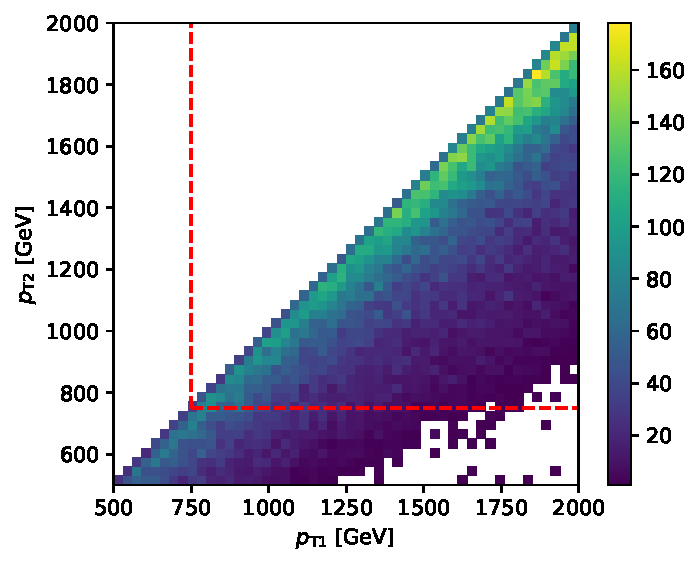
\includegraphics[width=0.45\textwidth]{HVmodel_pt_distribution-sig.pdf}
			}
			\subfloat[Background]{
				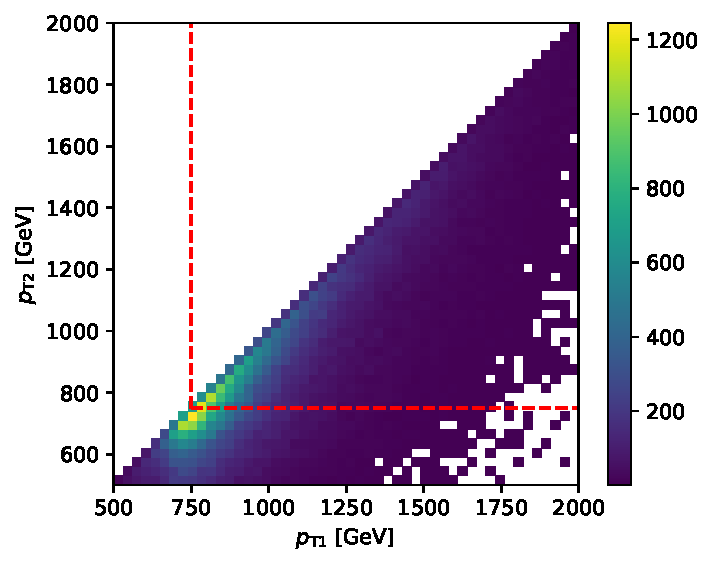
\includegraphics[width=0.45\textwidth]{HVmodel_pt_distribution-bkg.pdf}
			}
			\caption{The transverse momentum distribution of leading and sub-leading jets. The red dashed lines are the $p_{\text{T}}$ cut.}
			\label{fig:HVmodel_pt_distribution}
		\end{figure}

		\begin{figure}[htpb]
			\centering
			
			\subfloat[My plot]{
				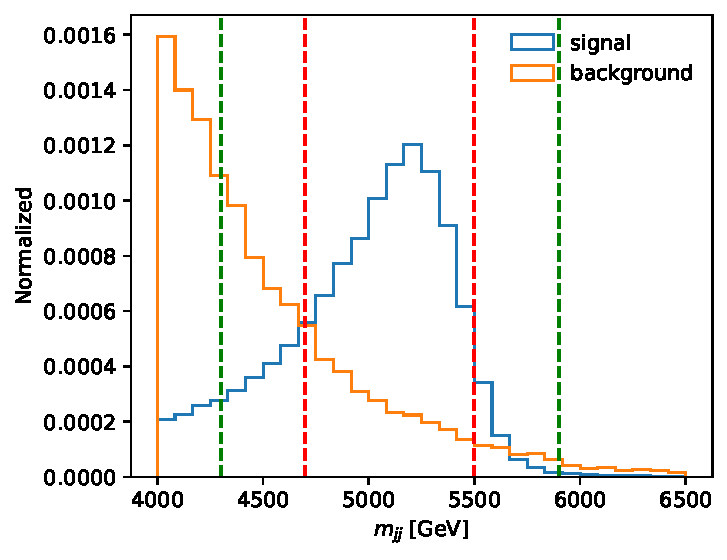
\includegraphics[width=0.45\textwidth]{HVmodel_mjj_distribution.pdf}
			}
			\subfloat[Zong-En's plot]{
				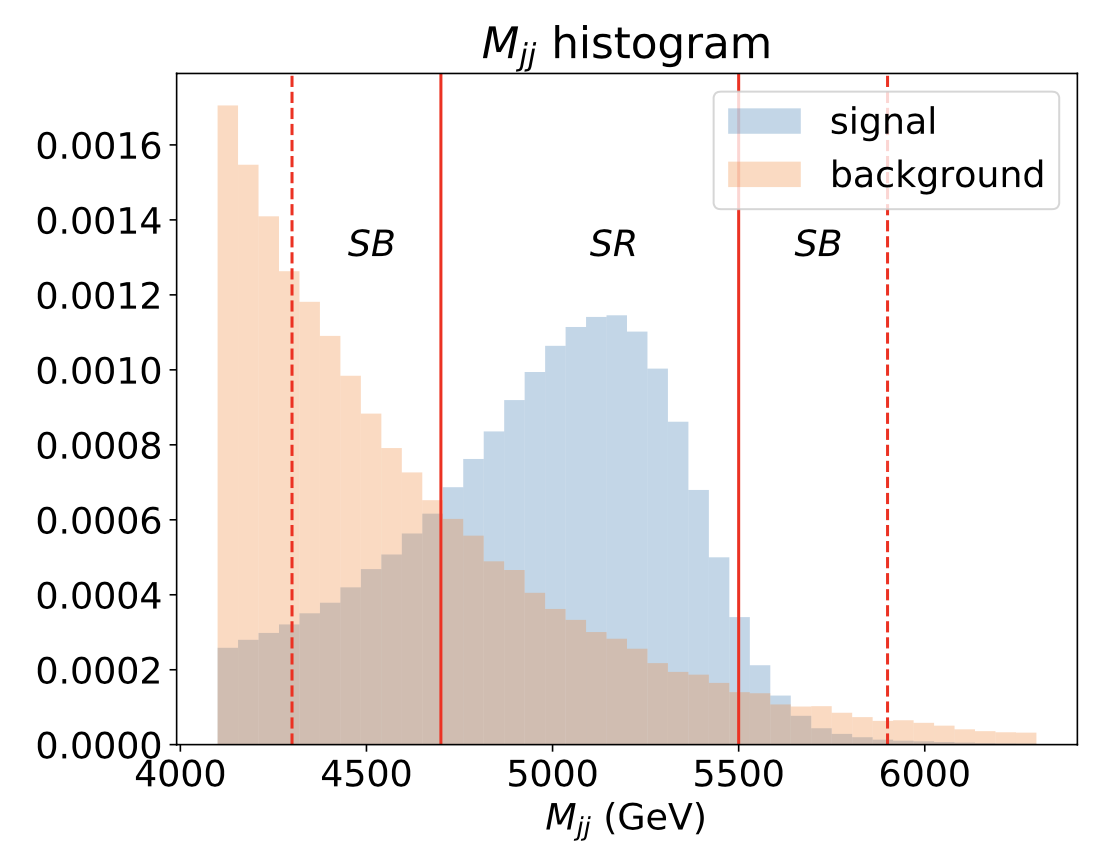
\includegraphics[width=0.50\textwidth]{HVmodel_mjj_distribution-Zong-En.png}
			}
			\caption{The total invriant mass $m_{jj}$ distribution of signal and background samples. In my plot, the signal region is between the red dashed lines. The sideband region is between the green dashed lines and excludes the signal region.}
			\label{fig:HVmodel_mjj_distribution}
		\end{figure}
	% subsection sample_selection (end)	
	\subsection{Jet image}% (fold)
	\label{sub:jet_image}
		We can construct the jet image from the event passing the selection cuts described in Section~\ref{sub:sample_selection}. The jet image is constructed for each jet separately, so for each event, we would obtain two jet images. They are treated as two channels of a picture. The following steps construct the jet image:
		\begin{enumerate}
			\item Centralization: Compute the $p_{\text{T}}$ weighted center in $\left( \eta,\phi \right) $ coordinates, then shift this point to origin.
			\item Rotation: Rotate the highest intensity axis to the $\eta$ axis.
			\item Flipping:	Flip the highest intensity quadrant to the first quadrant.
			\item Pixelating in $\eta \in [-1,1],\ \phi \in [-1,1]$ box, with $75\times 75$ pixels.
		\end{enumerate}

		Figure~\ref{fig:HVmodel_jet_image_one_event} is the jet images of a single event. Figure~\ref{fig:HVmodel_jet_image_average} is the average jet image. 

		\begin{figure}[htpb]
			\centering
			\subfloat[Signal]{
				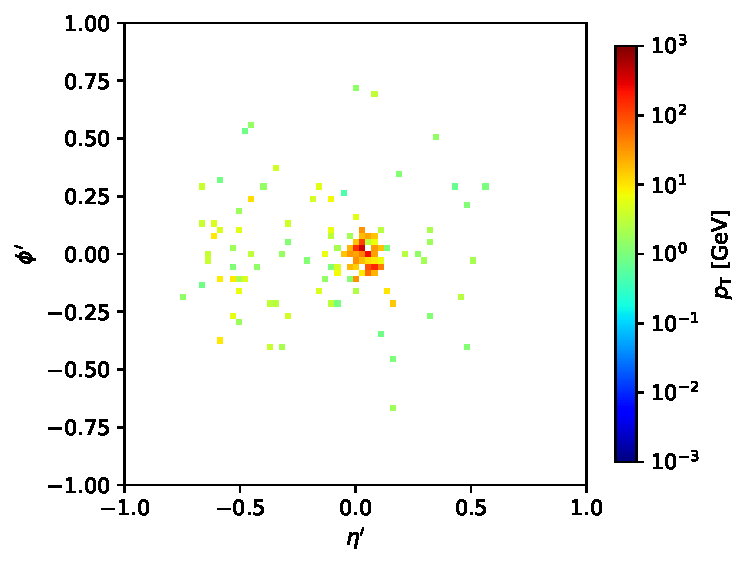
\includegraphics[width=0.45\textwidth]{HVmodel_signal_jet_image_one_event.pdf}
			}
			\subfloat[Background]{
				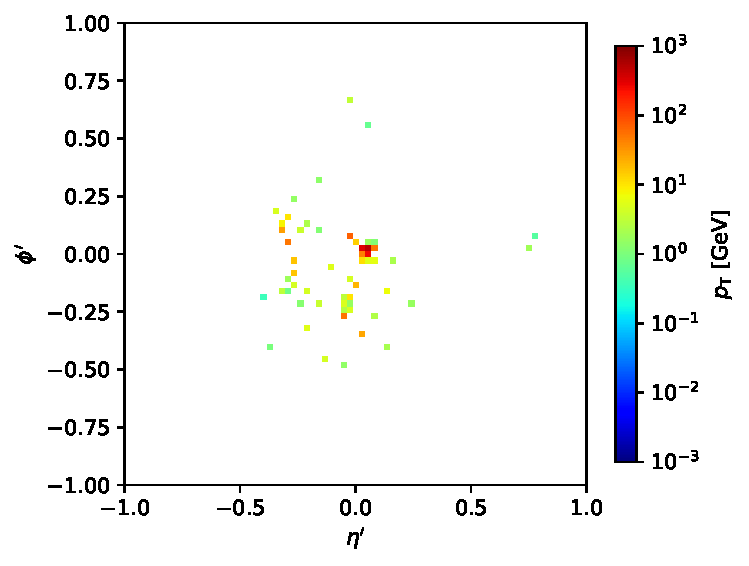
\includegraphics[width=0.45\textwidth]{HVmodel_background_jet_image_one_event.pdf}
			}
			\caption{The jet images of the leading jet in the signal region. The $\eta'$ and $\phi'$ are the coordinates after the preprocessing (centralization, rotation, flipping).}
			\label{fig:HVmodel_jet_image_one_event}
		\end{figure}
		\begin{figure}[htpb]
			\centering
			\subfloat[Signal]{
				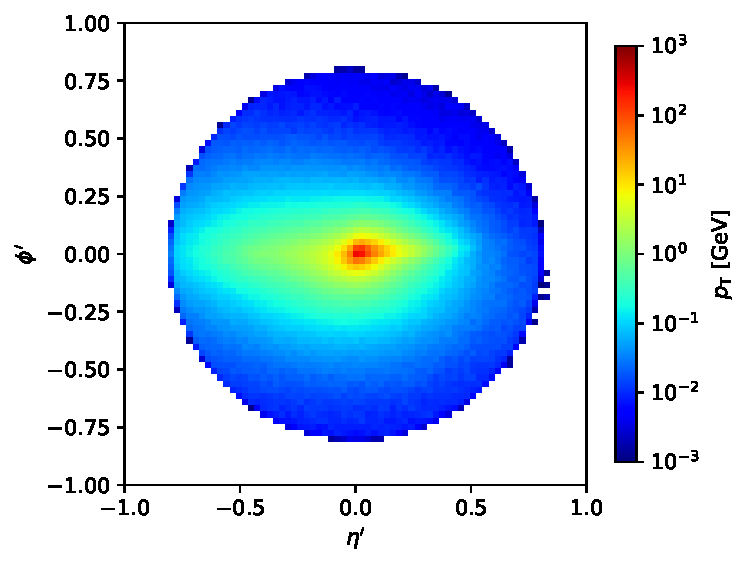
\includegraphics[width=0.45\textwidth]{HVmodel_signal_jet_image_average.pdf}
			}
			\subfloat[Background]{
				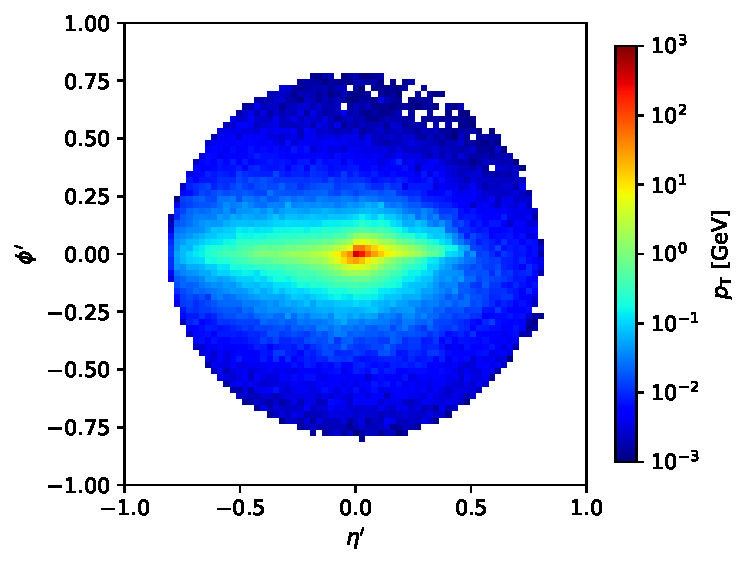
\includegraphics[width=0.45\textwidth]{HVmodel_background_jet_image_average.pdf}
			}
			\caption{The average jet images of the leading jet in the signal region. The $\eta'$ and $\phi'$ are the coordinates after the preprocessing (centralization, rotation, flipping). The number of the signal events is 56k. The number of the background events is 20k.}
			\label{fig:HVmodel_jet_image_average}
		\end{figure}
	% subsection jet_image (end)
	\subsection{Datasets}% (fold)
	\label{sub:datasets}
		The total cross-section of the background events is $6837 \text{ fb}$. From Table~\ref{tab:HVmodel_cutflow_number}, we can compute the corresponding cross-sections of signal and sideband regions are $136.1 \text{ fb}$ and $211.2 \text{ fb}$, respectively. Thus, the numbers of events in signal and sideband region are 19k and 29k at luminosity $\mathcal{L} = 139 \text{ fb}^{-1}$.

		The training sample sizes are summarized in Table~\ref{tab:training_sample_size_cwola_hunting_hv}.
		\begin{table}[htpb]
			\centering
			\caption{The training sample size for the mixed sample. We set sensitivity $S / \sqrt{B} = 1$ in the signal region and evaluate the number of events in the signal region. Then, the number of events in the sideband region can be obtained from Table~\ref{tab:HVmodel_cutflow_number}.}
			\label{tab:training_sample_size_cwola_hunting_hv}
			\begin{tabular}{c|cc}
								& \multicolumn{2}{c}{True label} \\
				Mixed sample    & Signal       & Background      \\ \hline
				Signal region   & 138          & 19k             \\
				Sideband region & 40           & 29k
			\end{tabular}
		\end{table}	

		The pure testing sample consists of 10k signal events and 10k background events, which are selected from the signal region.
	% subsection datasets (end)	
	\subsection{Training CNN}% (fold)
	\label{sub:training_cnn}
		The CNN model structure is summarized in Figure~\ref{fig:cnn_model_structure}. The internal node uses the rectified leaner unit (ReLU) as the activation function. The loss function is Categorical cross-entropy, and we use the Adam optimizer to optimize the loss function.
		\begin{figure}[htpb]
			\centering
			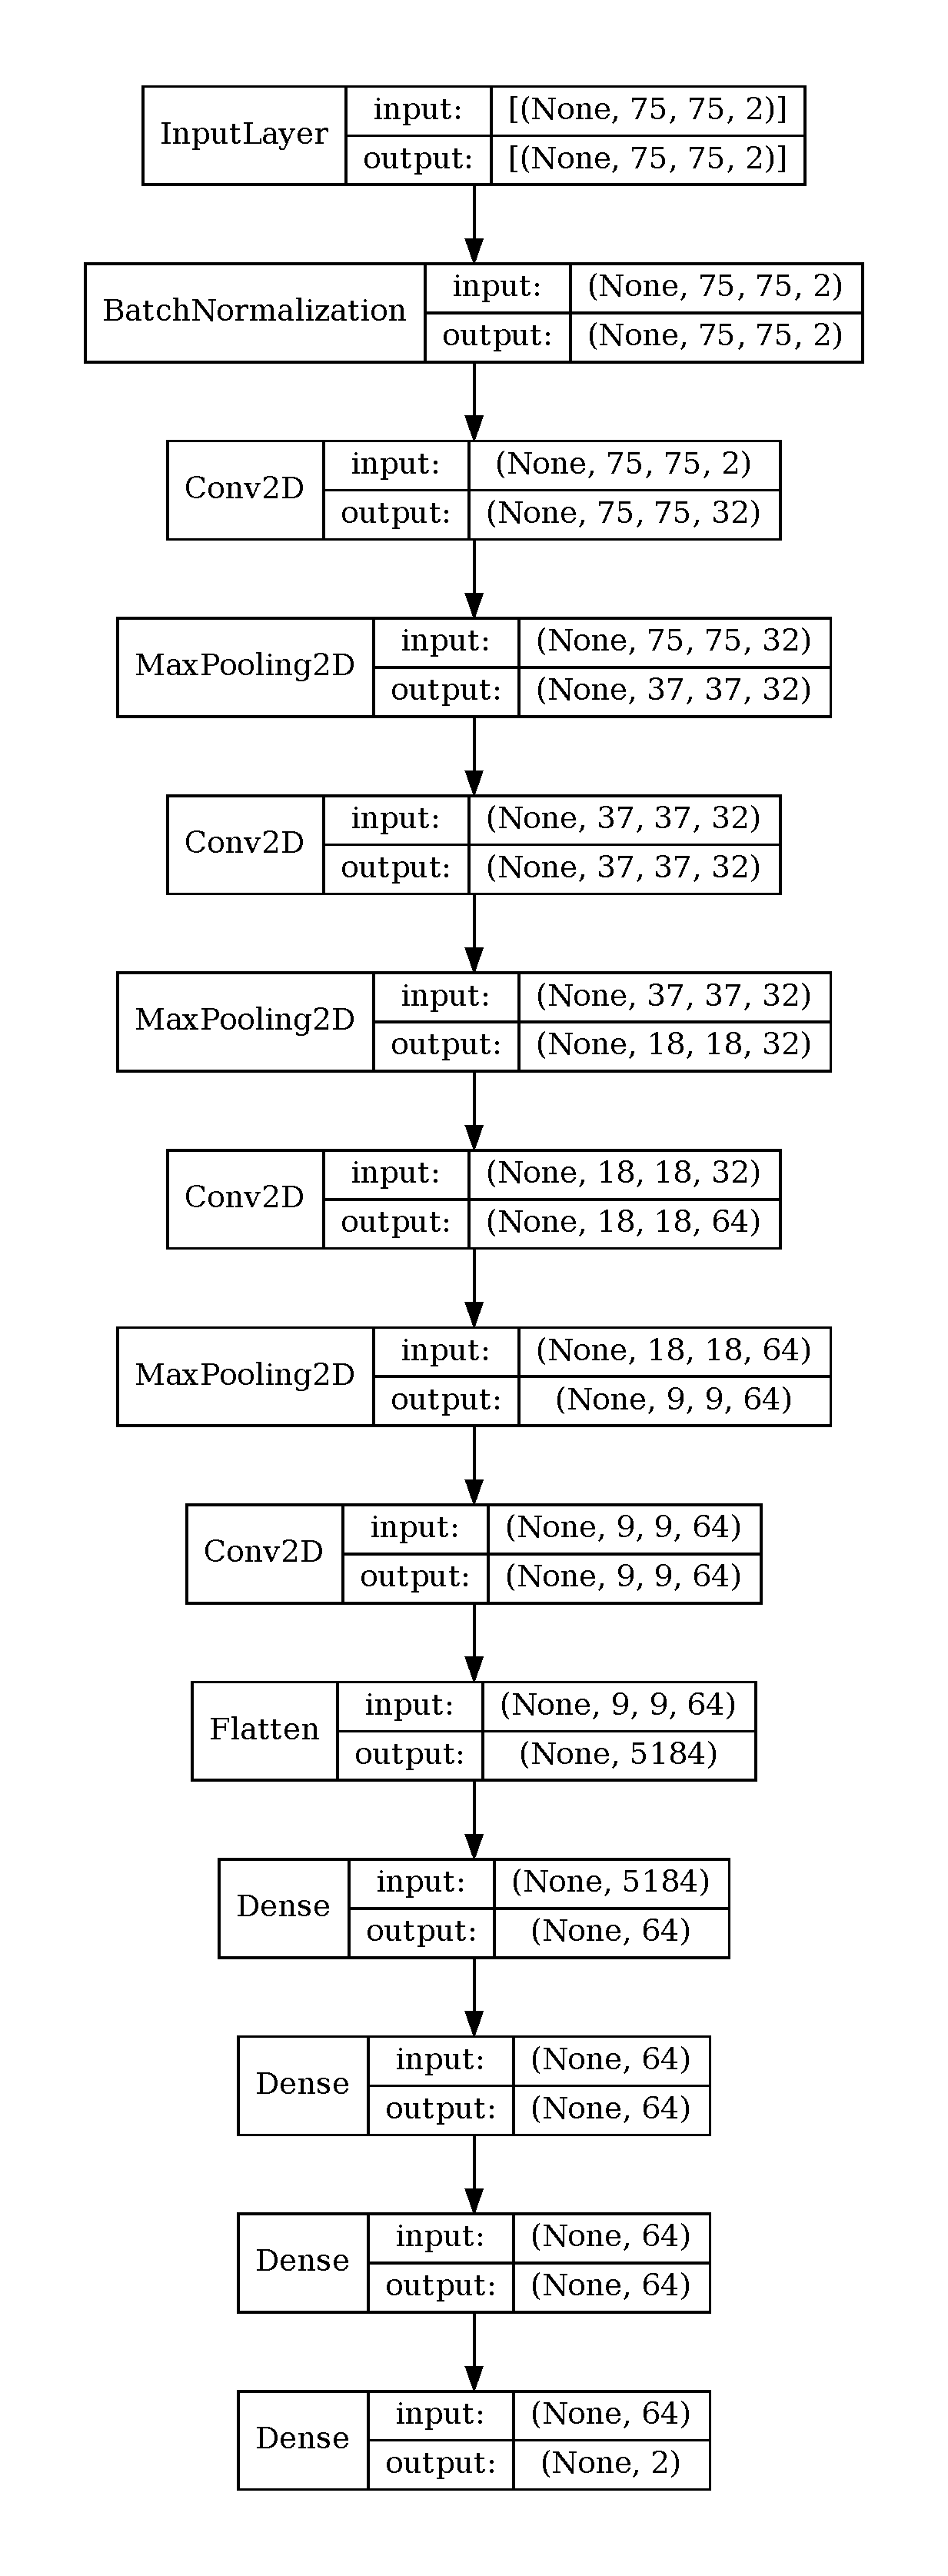
\includegraphics[width=0.45\textwidth]{CNN_model_structure.pdf}
			\caption{For first and second Conv2D layers, the kernel sizes are $5 \times 5$. For third and fourth Conv2D layers, the kernel sizes are $3 \times 3$.}
			\label{fig:cnn_model_structure}
		\end{figure}
	% subsection training_cnn (end)	
	\subsection{Hidden Valley model training results}% (fold)
	\label{sub:hidden_valley_model_training_results}
		The CNN is trained on samples with sensitivity $S / \sqrt{B}$ ranging from 1 to 10. Figure~\ref{fig:cwola_hunting_cnn_acc} presents the training results. These numbers are evaluated from the pure samples. The CNN cannot learn useful information for the case with a sensitivity $S / \sqrt{B} \le  5$, so the ACC is 0.5. After this region, the accuracy demonstrates a significant improvement. It seems that the CNN model surpasses a certain threshold.

		\begin{figure}[htpb]
			\centering
			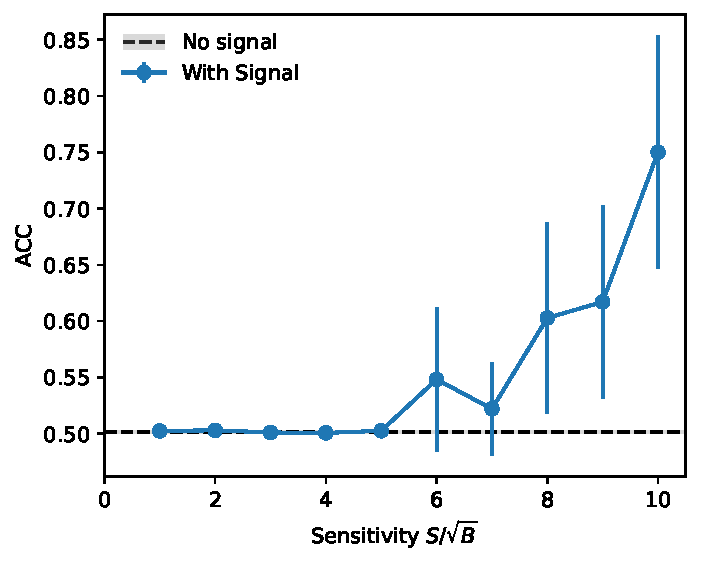
\includegraphics[width=0.55\textwidth]{HVmodel_CWoLa_CNN.pdf}
			\caption{The performance of CWoLa CNN training as a function of the sensitivity. The error bar is the standard deviation of 10 times training. The grey band is the error bar of the ``without signal'' case. For sensitivity less than 5, the error bar is too small to see.}
			\label{fig:cwola_hunting_cnn_acc}
		\end{figure}	
	% subsection hidden_valley_model_training_results (end)
	\subsection{Data process procedure}% (fold)
	\label{sub:data_process_procedure}
		\begin{enumerate}
			\item Generate the sample file in \verb|.root| format. Following Section~\ref{sub:sample_generation}.
			\item Apply the selection cuts described in Section~\ref{sub:sample_selection} and save the event passing the cuts in \verb|HDF5| format. The file contains the information listed below 
				\begin{itemize}
					\item The $\left( p_{\text{T}}, \eta, \phi \right) $ of leading and sub-leading jet constituents.
					\item Total invariant mass $m_{jj}$.
					\item Type of event: 1 for signal, 0 for background.	
				\end{itemize}
			\item Make mixed sample in \verb|HDF5| format. Following Section~\ref{sub:datasets}, we can compute the size of datasets.	
			\item Apply data augmentation in \verb|HDF5| format. Following Section~\ref{sub:data_augmentation}.
			\item Generate the jet image from \verb|HDF5| data.
		\end{enumerate}
		Note the preprocessing is done in step 5. If we do the preprocessing many times, then the rounding errors would break the jet image.
	% subsection data_process_procedure (end)	
	\subsection{Data augmentation}% (fold)
	\label{sub:data_augmentation}
		To reduce the threshold, the data augmentation technique is tested. Similar to the Section~\ref{sub:physical_augmentation}, we apply the $\eta-\phi$ smearing on our training sample. Specifically, the $\left( \eta,\phi \right) $ coordinate of jet constituents are resampled according to a Normal distribution centered on the original coordinate and with a standard deviation inversely proportional to the $p_{\text{T}}$
				\begin{equation}
					\eta' \sim \mathcal{N}\left(\eta, \frac{\Lambda}{p_{\text{T}}}\right), \quad \phi' \sim \mathcal{N}\left(\phi, \frac{\Lambda}{p_{\text{T}}}\right)
				\end{equation}
				where $\eta', \phi'$ are the augmented coordinate, $p_{\text{T}}$ is the transverse momentum of the jet constituent, and the smearing scale is set to be $\Lambda = \text{100 MeV}$.

		Figure~\ref{fig:eta_phi_smearing_jet_constituent_jet_image} and \ref{fig:eta_phi_smearing_phi_jet_constituent_average_jet_image} are the jet image before and after the augmentation. The jet images look similar before and after the augmentation, but not the same.
		\begin{figure}[htpb]
			\centering
			\subfloat[Before augmentation]{
				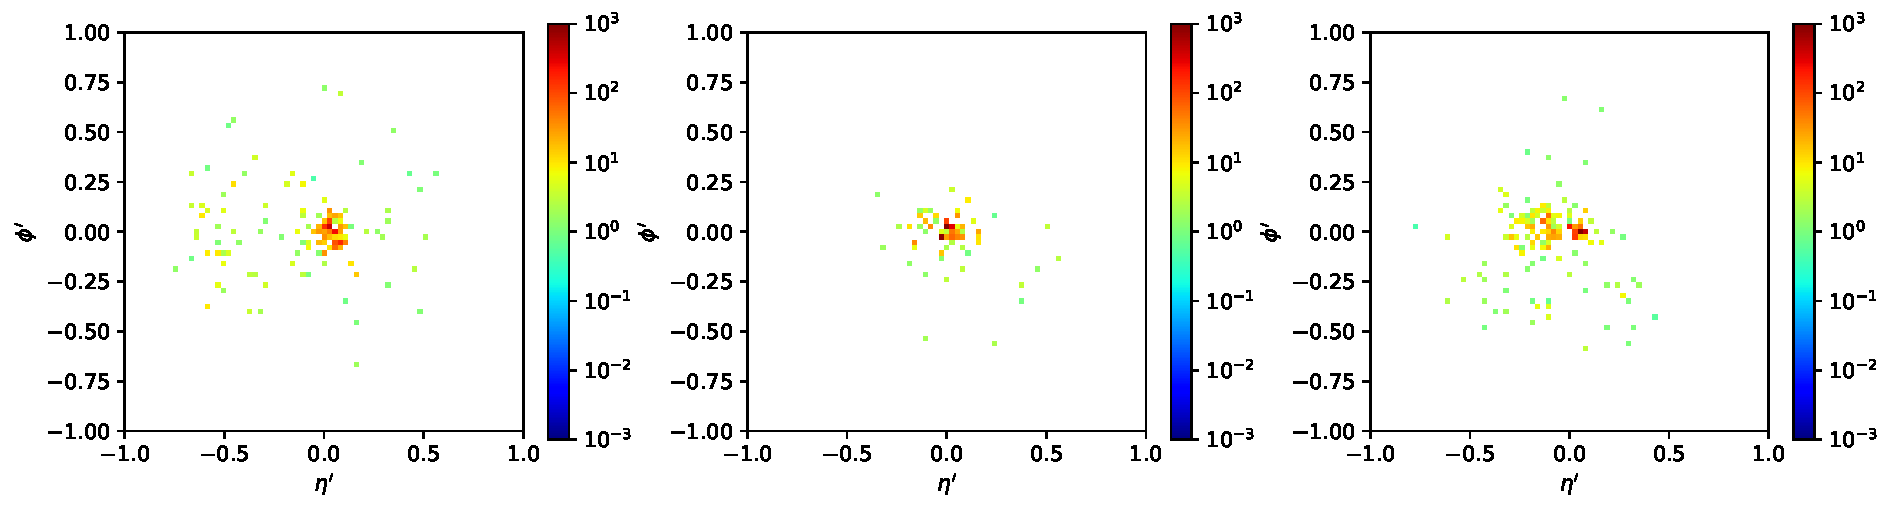
\includegraphics[width=0.95\textwidth]{HVmodel_jet_image_one_event_original.pdf}
			} \\
			\subfloat[After augmentation]{
				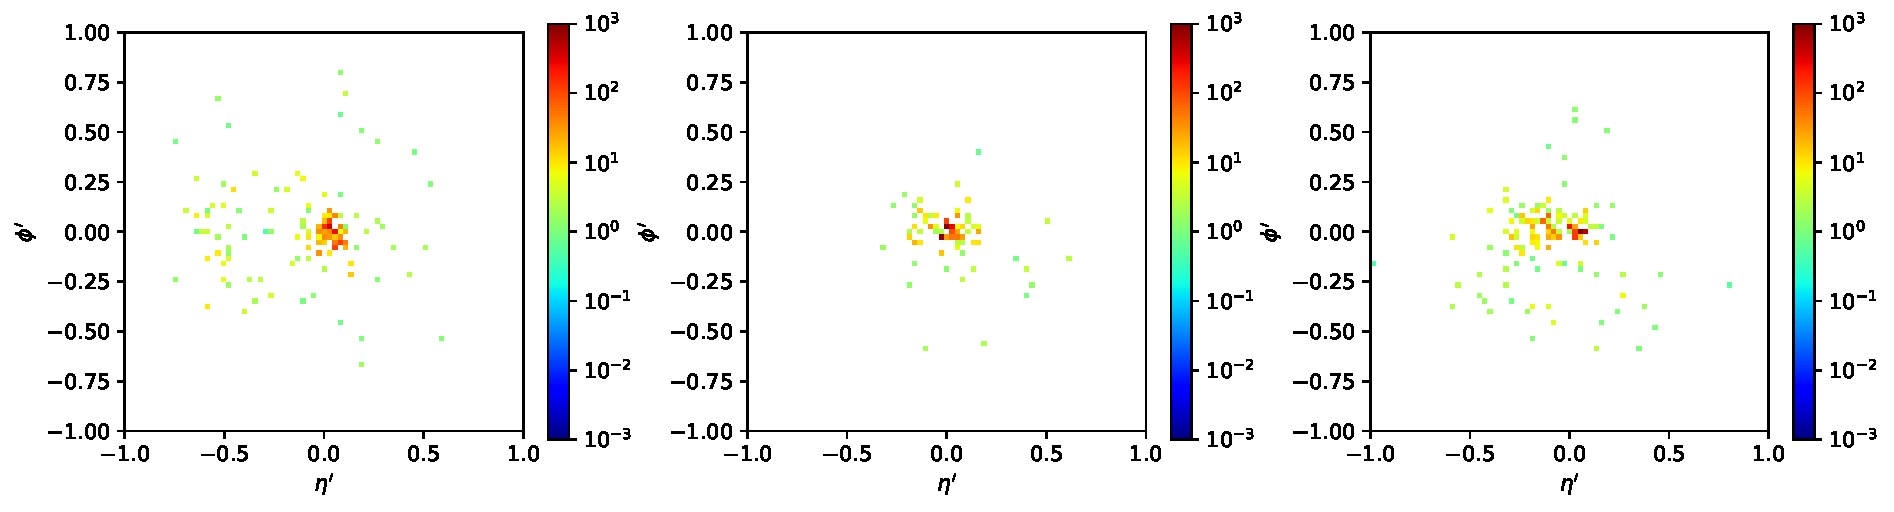
\includegraphics[width=0.95\textwidth]{HVmodel_jet_image_one_event_eta_phi_smearing.pdf}
			}
			\caption{The jet images before and after the $\eta-\phi$ smearing augmentation.}
			\label{fig:eta_phi_smearing_jet_constituent_jet_image}
		\end{figure}
		\begin{figure}[htpb]
			\centering
			\subfloat[Before augmentation]{
				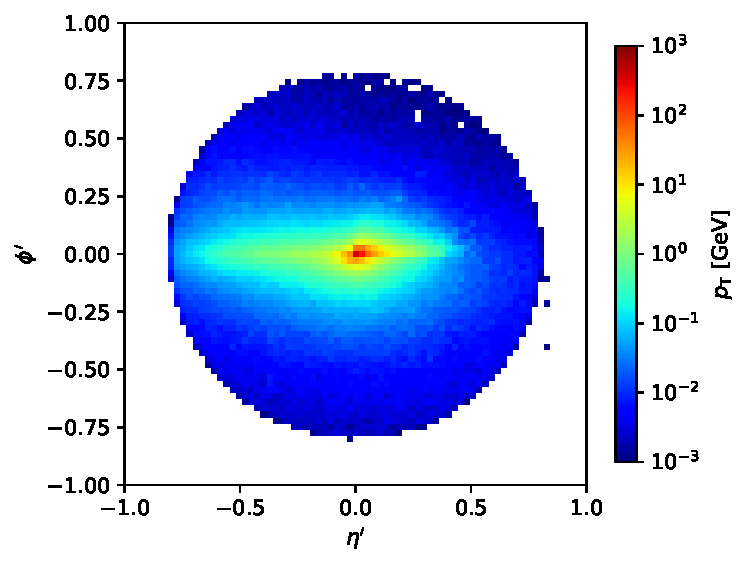
\includegraphics[width=0.45\textwidth]{HVmodel_jet_image_average_original.pdf}
			}
			\subfloat[After augmentation]{
				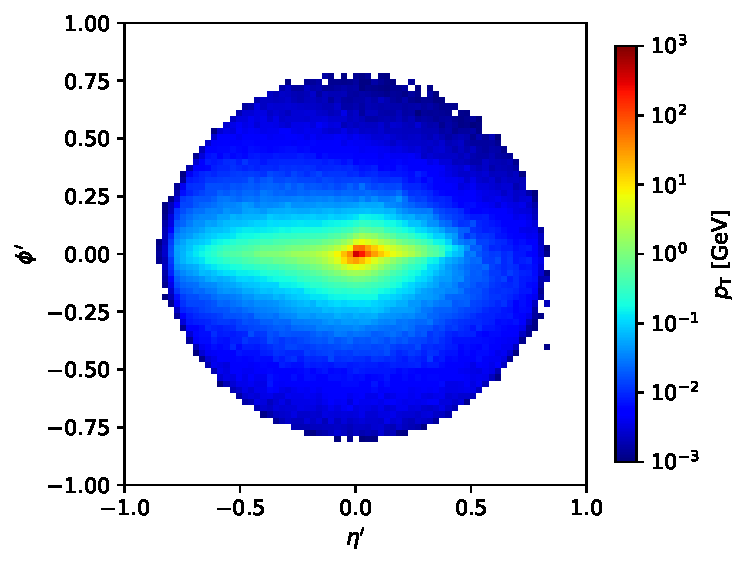
\includegraphics[width=0.45\textwidth]{HVmodel_jet_image_average_aug_1.pdf}
			}
			\caption{The average jet images before and after the $\eta-\phi$ smearing augmentation.}
			\label{fig:eta_phi_smearing_phi_jet_constituent_average_jet_image}
		\end{figure}
		
		We generate samples with sensitivity $S / \sqrt{B}$ ranging from 1 to 10. Then, apply the data augmentation to make larger samples. These samples are used for CNN training. Figure~\ref{fig:cwola_hunting_cnn_acc_data_augmetation} presents the training results. These numbers are evaluated from the pure samples. The ACC is better than previous results (blue curve in Figure~\ref{fig:cwola_hunting_cnn_acc}) for the ``+1 times'' curve for all sensitivities. The data augmentation technique seems to suppress the threshold and improve the training performance.

		\begin{figure}[htpb]
			\centering
			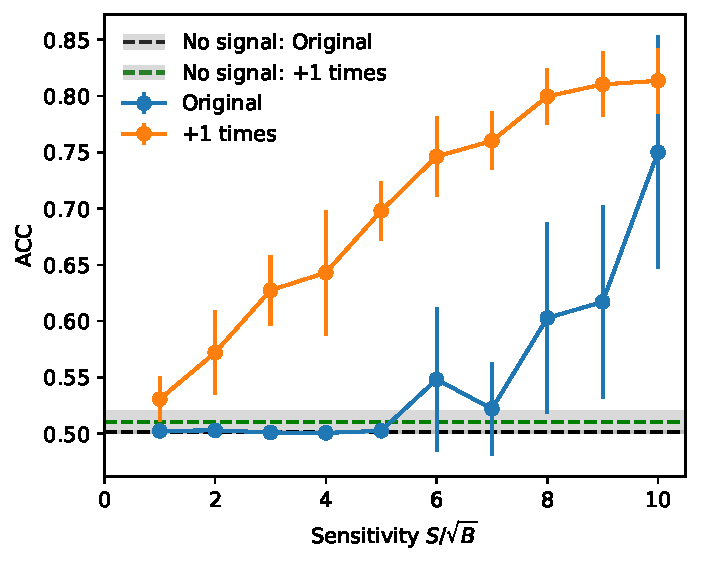
\includegraphics[width=0.55\textwidth]{HVmodel_CWoLa_CNN_aug_1.pdf}
			\caption{The performance of CWoLa CNN training as a function of the sensitivity. The error bar is the standard deviation of 10 times training. The grey band is the error bar of the ``without signal'' case.}
			\label{fig:cwola_hunting_cnn_acc_data_augmetation}
		\end{figure}

		 Figure~\ref{fig:cwola_hunting_cnn_acc_data_augmetation_3_times} presents the training results with larger samples. For the ``+3 times'' curve, there is a strange result, the ACC is worse than the ``+1 times'' case for sensitivities $S / \sqrt{B} \ge 3$. There are some problems in the training procedure, e.g. overfitting.
		\begin{figure}[htpb]
			\centering
			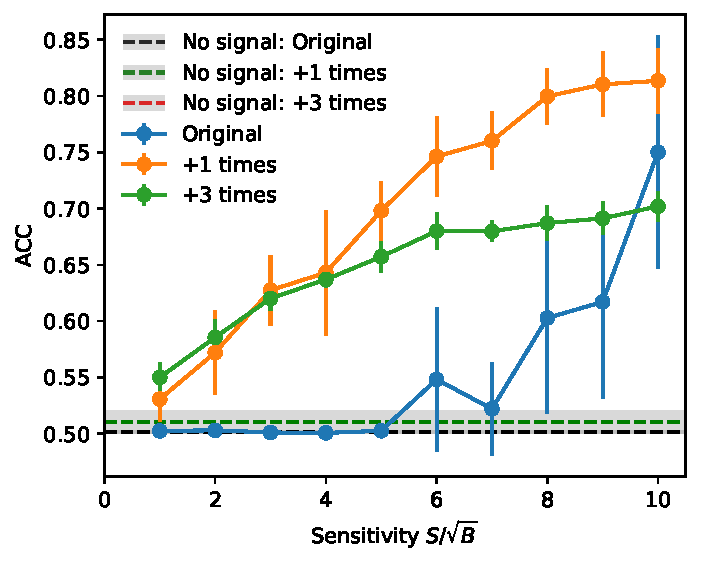
\includegraphics[width=0.55\textwidth]{HVmodel_CWoLa_CNN_aug_1_3.pdf}
			\caption{The performance of CWoLa CNN training as a function of the sensitivity. The error bar is the standard deviation of 10 times training. The grey band is the error bar of the ``without signal'' case.}
			\label{fig:cwola_hunting_cnn_acc_data_augmetation_3_times}
		\end{figure}

		 Figure~\ref{fig:eta_phi_smearing_phi_jet_constituent_average_jet_image_aug_1_3} shows the average jet image for different augmentation times.
		 \begin{figure}[htpb]
			\centering
			\subfloat[+1 times]{
				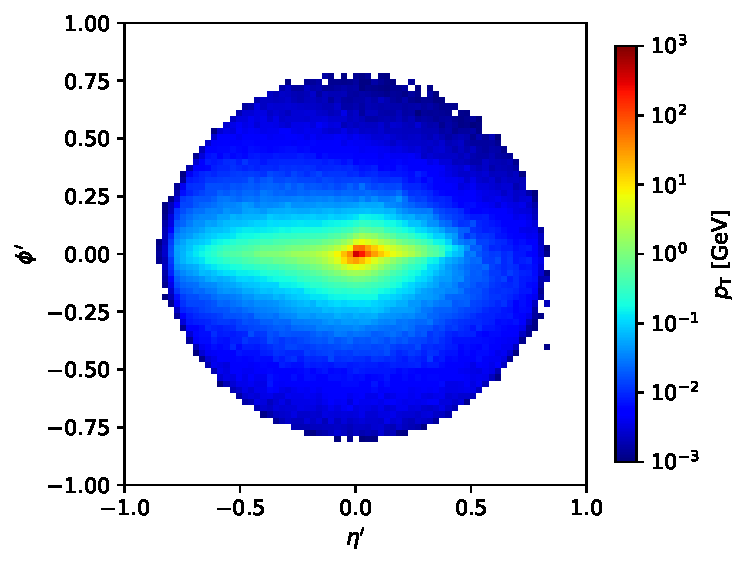
\includegraphics[width=0.45\textwidth]{HVmodel_jet_image_average_aug_1.pdf}
			}
			\subfloat[+3 times]{
				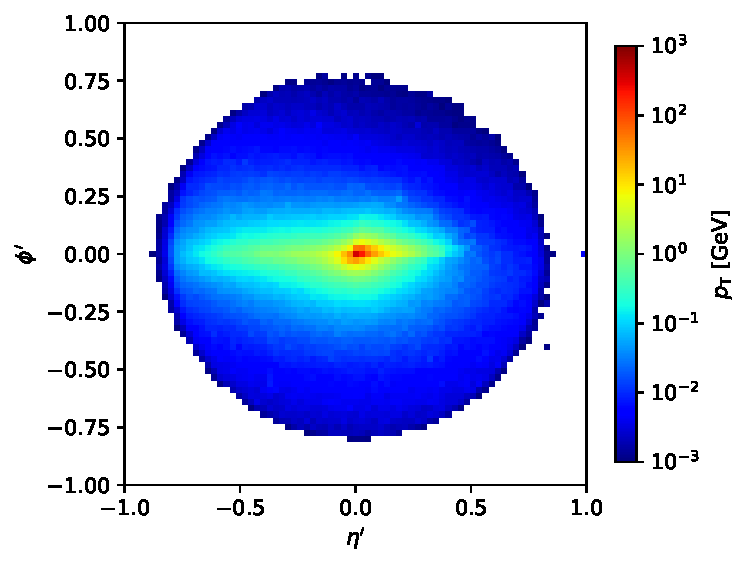
\includegraphics[width=0.45\textwidth]{HVmodel_jet_image_average_aug_3.pdf}
			}
			\caption{The average jet images of the $\eta-\phi$ smearing augmentation with different times.}
			\label{fig:eta_phi_smearing_phi_jet_constituent_average_jet_image_aug_1_3}
		\end{figure}
	% subsection data_augmentation (end)	
	\subsection{Enlarge the training sample size}% (fold)
	\label{sub:enlarge_the_training_sample_size}
		To validate the correctness of the data augmentation results, we generated larger samples by scaling the luminosity. To compare the results with ``+1 times'' augmentation, we scale the luminosity to $\mathcal{L} = 139 \times 2 \text{ fb}^{-1}$. It is important to note that the number of signal events is not equal for ``+1 times'' and ``luminosity $\times 2$'' at the same sensitivity because the number of signal events is computed from $S / \sqrt{B}$ for a given $B$, resulting in the number of ``+1 times'' signal sample is greater by a factor of $\sqrt{2}$. Table~\ref{tab:training_sample_size_cwola_hunting_hv_aug_1_x2_luminosity} is an example. For a fair comparison, where the sizes of signal and background events are the same, we should compare the ``+1 times'' results with the point on the ``luminosity $\times 2$'' curve corresponding to $\sqrt{2}$ times the sensitivity.

		\begin{table}[htpb]
			\centering
			\caption{The training sample size for the original, ``+1 times'' and ``luminosity $\times 2$'' mixed sample. We set sensitivity $S / \sqrt{B} = 1$ in the signal region and evaluate the number of events in the signal region.}
			\label{tab:training_sample_size_cwola_hunting_hv_aug_1_x2_luminosity}
			
			\begin{tabular}{c|cc|cc|cc}
								& \multicolumn{2}{c|}{Original}& \multicolumn{2}{c|}{+1 times}& \multicolumn{2}{c}{luminosity $\times 2$} \\
				Mixed sample    & Signal      & Background     & Signal      & Background     & Signal            & Background            \\ \hline
				Signal region   & 138         & 19k            & 276         & 38k            & 194               & 38k                   \\
				Sideband region & 40          & 29k            & 80          & 58k            & 56                & 58k                  
			\end{tabular}
		\end{table}
		
		Figure~\ref{fig:cwola_hunting_cnn_acc_x2_luminosity} presents the training results with larger samples. The results of ``luminosity $\times 2$'' is better than the original sample, but still worse than the ``+1 times'' case. Even considering the $\sqrt{2}$ scale factor, the corresponding points' performance is still worse. There may be something wrong with the data processing or training codes.
		\begin{figure}[htpb]
			\centering
			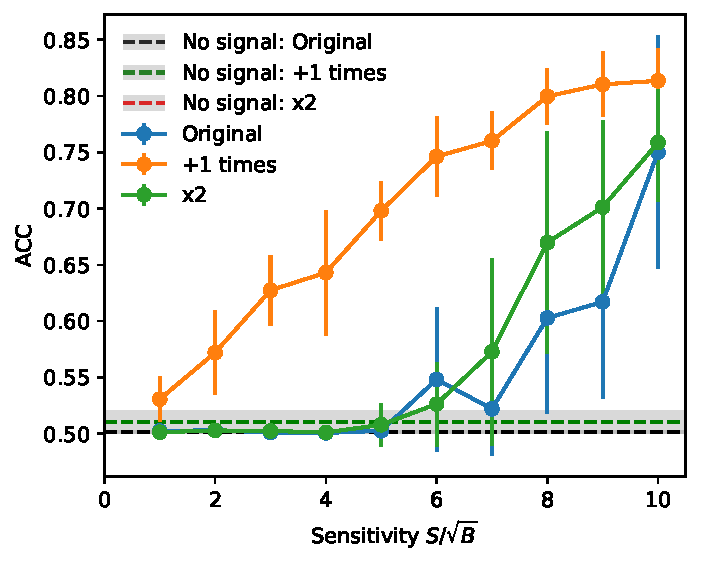
\includegraphics[width=0.55\textwidth]{HVmodel_CWoLa_CNN_aug_1_x2.pdf}
			\caption{The performance of CWoLa CNN training as a function of the sensitivity. The error bar is the standard deviation of 10 times training. The grey band is the error bar of the ``without signal'' case.}
			\label{fig:cwola_hunting_cnn_acc_x2_luminosity}
		\end{figure}
	% subsection enlarge_the_training_sample_size (end)
	\subsection{Check the codes and make more plots}% (fold)
	\label{sub:check_the_codes_and_make_more_plots}
		The data process steps from 2 to 5 (Section~\ref{sub:data_process_procedure}) have been checked and samples are processed again.

		Figure~\ref{fig:jet_constituent_pt_distribution} is the $p_\text{T}$ distribution of the jet constituents. The distributions of leading and sub-leading jet constituents are similar.
		\begin{figure}[htpb]
			\centering
			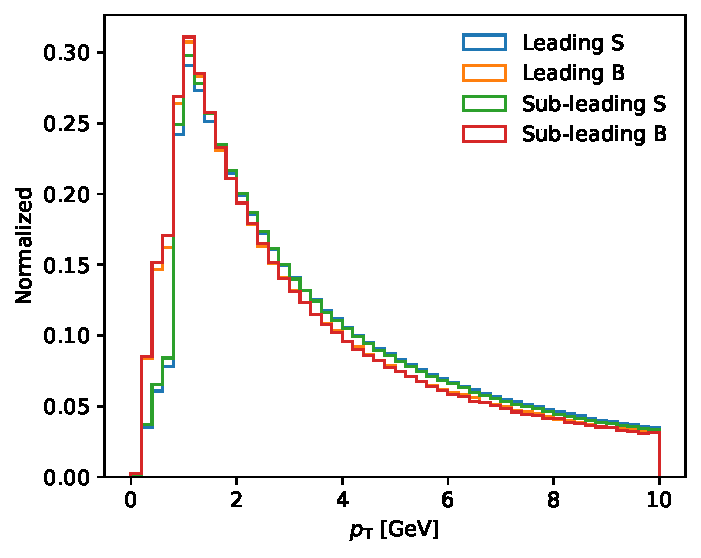
\includegraphics[width=0.55\textwidth]{hv_model_pt_distribution.pdf}
			\caption{The transverse momentum distribution of jet constituents.}
			\label{fig:jet_constituent_pt_distribution}
		\end{figure}

		Figure~\ref{fig:jet_constituent_eta_distribution} and \ref{fig:jet_constituent_phi_distribution} are the $\eta, \phi$ distributions before and after the augmentation. Because the smearing scale is small, the distributions look almost the same for both cases.

		\begin{figure}[htpb]
			\centering
			\subfloat[Leading Higgs]{
				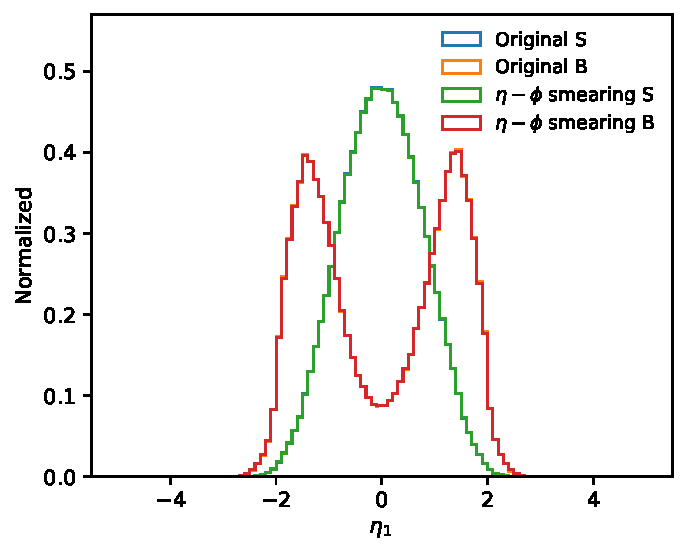
\includegraphics[width=0.45\textwidth]{hv_model_eta1_distribution_eta_phi_smearing.pdf}
			}
			\subfloat[Sub-leading Higgs]{
				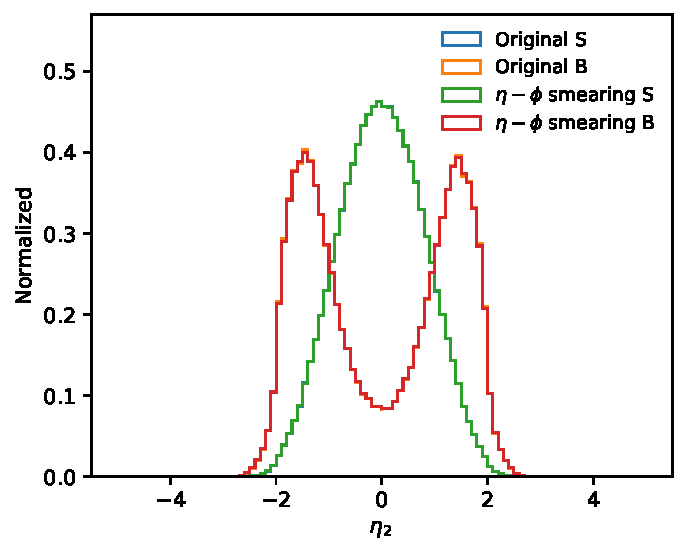
\includegraphics[width=0.45\textwidth]{hv_model_eta2_distribution_eta_phi_smearing.pdf}
			}
			\caption{The pseudorapidity distribution before and after the $\eta-\phi$ smearing augmentation. $\eta_1$ and $\eta_2$ are the pseudorapidities of the leading and sub-leading jet constituents.}
			\label{fig:jet_constituent_eta_distribution}
		\end{figure}
		\begin{figure}[htpb]
			\centering
			\subfloat[Leading Higgs]{
				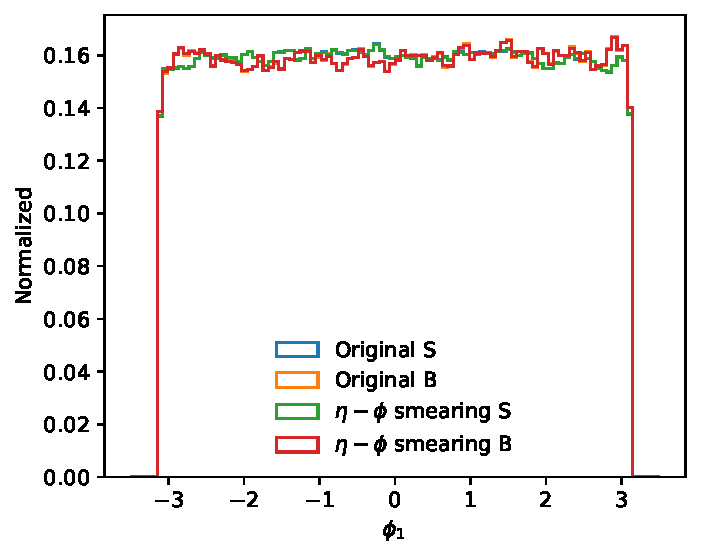
\includegraphics[width=0.45\textwidth]{hv_model_phi1_distribution_eta_phi_smearing.pdf}
			}
			\subfloat[Sub-leading Higgs]{
				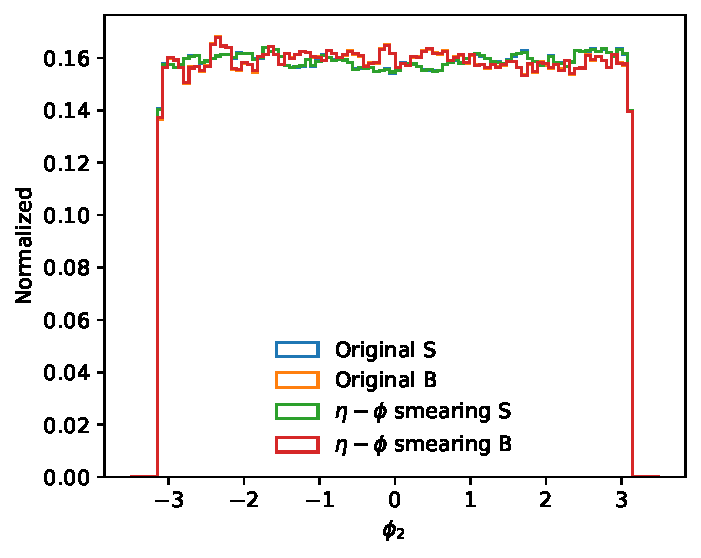
\includegraphics[width=0.45\textwidth]{hv_model_phi2_distribution_eta_phi_smearing.pdf}
			}
			\caption{The azimuthal angle distribution before and after the $\eta-\phi$ smearing augmentation. $\phi_1$ and $\phi_2$ are the azimuthal angles of the leading and sub-leading jet constituents.}
			\label{fig:jet_constituent_phi_distribution}
		\end{figure}

		Figure~\ref{fig:jet_constituent_average_jet_image_aug_1_x2} shows the average jet image for various cases.
		\begin{figure}[htpb]
			\centering
			\subfloat[Original]{
				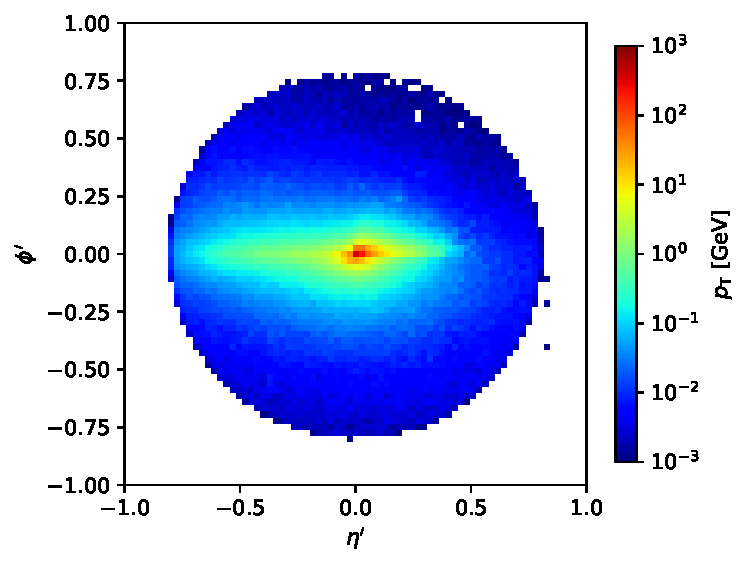
\includegraphics[width=0.32\textwidth]{HVmodel_jet_image_average_original.pdf}
			}
			\subfloat[+1 times augmentation]{
				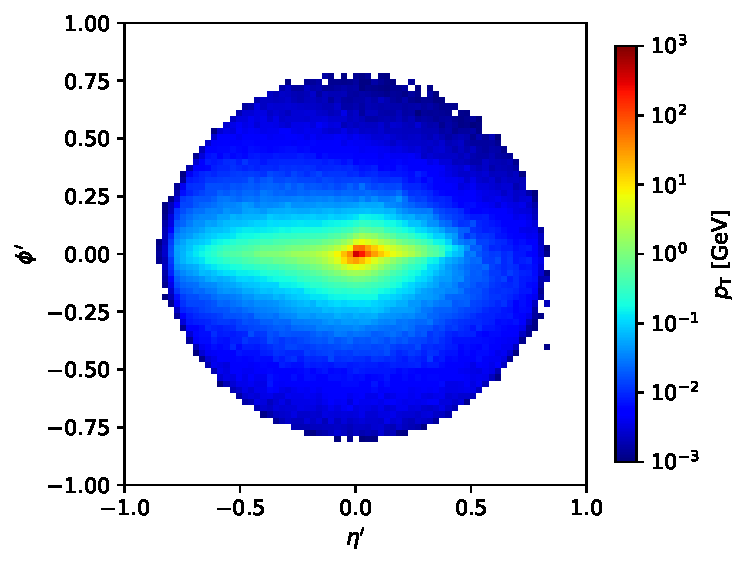
\includegraphics[width=0.32\textwidth]{HVmodel_jet_image_average_aug_1.pdf}
			}
			\subfloat[Luminosity $\times 2$]{
				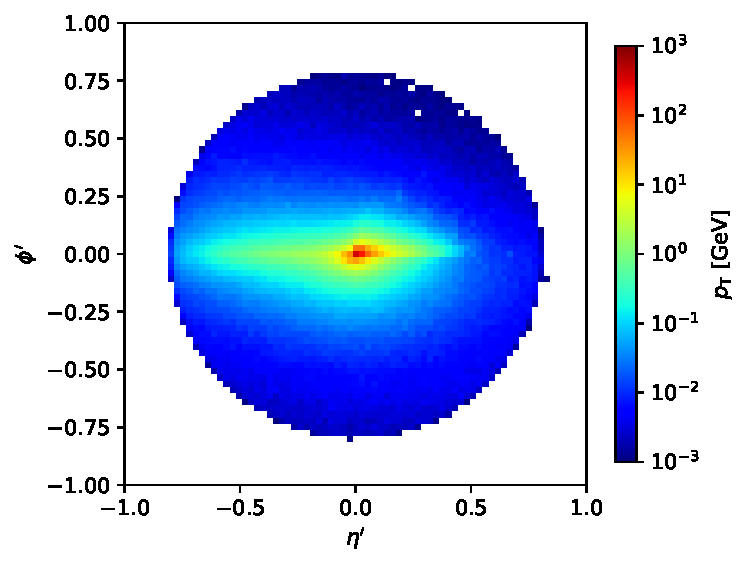
\includegraphics[width=0.32\textwidth]{HVmodel_jet_image_average_x2.pdf}
			}
			\caption{The average jet images of different cases. These plots are made from mixed samples.}
			\label{fig:jet_constituent_average_jet_image_aug_1_x2}
		\end{figure}

		Figure~\ref{fig:cwola_hunting_cnn_acc_x2_luminosity_re-processed_sample} is training results with re-processed samples.
		\begin{figure}[htpb]
			\centering
			\includegraphics[width=0.55\textwidth]{HVmodel_CWoLa_CNN_aug_1_x2_re-process.pdf}
			\caption{The performance of CWoLa CNN training with re-processed samples. The error bar is the standard deviation of 10 times training. The grey band is the error bar of the ``without signal'' case.}
			\label{fig:cwola_hunting_cnn_acc_x2_luminosity_re-processed_sample}
		\end{figure}
	% subsection check_the_codes_and_make_more_plots (end)
	\subsection{Sensitivity difference}% (fold)
	\label{sub:sensitivity_difference}
		The CWoLa CNN is applied for event selection. The threshold is set for a given background efficiency $\varepsilon_{\text{b}}$ (false positive rate). For a given $\varepsilon_b$, the sensitivity would be scale by a factor ${\varepsilon_\text{s}} / {\sqrt{\varepsilon_{\text{b}}}}$.

		Figure~\ref{fig:sensitivity_improvement_origin_aug_1_x2} is the sensitivity improvement of orginal, ``+1 times'' and ``luminosity $\times 2$'' samples. The $10\%$ curves give more stable results. The lower background efficiencies could achieve better results at the range with higher sensitivities, but the standard deviation would be much larger. Figure~\ref{fig:sensitivity_improvement_bkg_eff_01} compares the sensitivity improvement of various training samples with the same background efficiency. The ``+1 times'' samples provide the best threshold among all.

		\begin{figure}[htpb]
			\centering
			\subfloat[Original]{
				\includegraphics[width=0.32\textwidth]{HVmodel_sensitivity_improvement_original.pdf}
			}
			\subfloat[+1 times augmentation]{
				\includegraphics[width=0.32\textwidth]{HVmodel_sensitivity_improvement_aug_1.pdf}
			}
			\subfloat[Luminosity $\times 2$]{
				\includegraphics[width=0.32\textwidth]{HVmodel_sensitivity_improvement_x2.pdf}
			}
			\caption{The sensitivities before and after the CWoLa CNN selection. The thresholds are chosen from $\varepsilon_{\text{b}} = 10\%, 1\%, 0.1\%$. The slope of the dashed line is $1$, representing the same performance before and after the selection. The error bar is the standard deviation of 10 times training.}
			\label{fig:sensitivity_improvement_origin_aug_1_x2}
		\end{figure}

		\begin{figure}[htpb]
			\centering
			\includegraphics[width=0.55\textwidth]{HVmodel_sensitivity_improvement_bkg_eff_10.pdf}
			\caption{The sensitivities before and after the CWoLa CNN selection. The threshold is chosen from $\varepsilon_{\text{b}} = 10\%$. The slope of the dashed line is $1$, representing the same performance before and after the selection. The error bar is the standard deviation of 10 times training. The ``+1 times'' samples provide the best threshold.}
			\label{fig:sensitivity_improvement_bkg_eff_01}
		\end{figure}
	% subsection sensitivity_difference (end)
	\subsection{Training and true performance}% (fold)
	\label{sub:training_and_true_performance}
		In our intuition, we would expect that``+1 times'' and ``luminosity  $\times 2$'' samples should exhibit similar performance, or the ``luminosity  $\times 2$'' sample might provide better results since the data augmentation generates more samples from the known data. However, the results in Figure~\ref{fig:sensitivity_improvement_bkg_eff_01} contradict our intuition. Since we use the CWoLa approach, our comparison is not based on the training performance on mixed samples; instead, we evaluate the testing performance on pure samples, referred to as ``true performance.'' The relationship between training and true performance may not be a monotonic function and can be quite complicated.

		Figure~\ref{fig:training_and_true_acc_ori_aug_1_x2} is the scatter plot for training and true accuracy. Training ACC values are close for all cases, but true ACC values can be much different. The true ACC has a range that is ten times larger than the training ACC range. For training ACC, both ``+1 times'' and ``luminosity $\times 2$'' samples show similar performance, slightly better than the original results. For the true ACC, the ``+1 times'' provides much better results. It seems that ``+1 times'' samples are more effective in improving true ACC.
		\begin{figure}[htpb]
			\centering
			\includegraphics[width=0.55\textwidth]{HVmodel_training_true_acc_aug_1_x2.pdf}
			\caption{Scatter plot for training ACC and true ACC. The slope of the grey dashed line is $1$, representing the same training and true ACC. The range of training ACC is very small, roughly 0.03, while the range of true ACC is about 0.3.}
			\label{fig:training_and_true_acc_ori_aug_1_x2}
		\end{figure}

		Figure~\ref{fig:training_and_true_acc_ori_aug_1_3_x2} includes results with``+3 times'' training . The ``+3 times'' samples provide much better training ACC, but they do not achieve higher performance for true ACC.
		\begin{figure}[htpb]
			\centering
			\includegraphics[width=0.55\textwidth]{HVmodel_training_true_acc_aug_1_3_x2.pdf}
			\caption{Scatter plot for training ACC and true ACC. The slope of the grey dashed line is $1$, representing the same training and true ACC.}
			\label{fig:training_and_true_acc_ori_aug_1_3_x2}
		\end{figure}
	% subsection training_and_true_performance (end)
	\subsection{Miscellaneous test}% (fold)
	\label{sub:miscellaneous_test}
		\subsubsection{Sensitivity 11 to 20}% (fold)
		\label{subs:sensitivity_11_to_20}
			To find out the training performance when sensitivity is greater than 10, we generate the samples with sensitivity ranging from 11 to 20. The training performance is summarized in Figure~\ref{fig:cwola_cnn_training_performance_11_20}. The ACC is increased when the sensitivity is increased. When the $S / \sqrt{B} > 13$, the ACC improvement is slowed down, where the ACC is 85\%. The training ACC is still similar for all cases, but the true ACC exhibits better value when the sensitivity is higher.
			\begin{figure}[htpb]
				\centering
				\subfloat[]{
					\includegraphics[width=0.45\textwidth]{HVmodel_CWoLa_CNN_sensitivity_11_20.pdf}
				}
				\subfloat[]{
					\includegraphics[width=0.45\textwidth]{HVmodel_training_true_acc_sensitivity_11_20.pdf}
				}
				\caption{(a) The performance of CWoLa CNN training with higher sensitivity samples. The error bar is the standard deviation of 10 times training. The grey band is the error bar of the ``without signal'' case. (b) Scatter plot for training ACC and true ACC. The slope of the grey dashed line is 1, representing the same training and true ACC.}
				\label{fig:cwola_cnn_training_performance_11_20}
			\end{figure}
		% subsubsection sensitivity_11_to_20 (end)
		\subsubsection{+1 copy sample}% (fold)
		\label{subs:_1_copy_sample}
			To investigate the impact of the data augmentation technique, we generate a sample by duplicating the original sample without any augmentation. This sample is called ``+1 copy.''
			Figure~\ref{fig:cwola_cnn_training_performance_copy_1} is the ACC curve and ACC distribution. The ACC is close ``+1 augmentation'' case when $S / \sqrt{B} \le 4$, while the ACC is worse when $S / \sqrt{B} \ge 5$. The training ACC is much better than the original and ``+1 augmentation'' samples, but the true ACC can not achieve higher values.
			\begin{figure}[htpb]
				\centering
				\subfloat[]{
					\includegraphics[width=0.45\textwidth]{HVmodel_CWoLa_CNN_aug_1_copy_1.pdf}
				}
				\subfloat[]{
					\includegraphics[width=0.45\textwidth]{HVmodel_training_true_acc_aug_1_copy_1.pdf}
				}
				\caption{(a) The performance of CWoLa CNN training with ``+1 copy'' samples. The error bar is the standard deviation of 10 times training. The grey band is the error bar of the ``without signal'' case. (b) Scatter plot for training ACC and true ACC. The slope of the grey dashed line is 1, representing the same training and true ACC.}
				\label{fig:cwola_cnn_training_performance_copy_1}
			\end{figure}

			Figure~\ref{fig:sensitivity_improvement_bkg_eff_01_copy_1} is the sensitivity improvement. The performance of the ``+1 copy'' sample is worse than ``+1 augmentation''. It exhibits the worst results in high-sensitivity regions. The data augmentation is effective in improving the true ACC.
			\begin{figure}[htpb]
				\centering
				\includegraphics[width=0.55\textwidth]{HVmodel_sensitivity_improvement_bkg_eff_10_copy_1.pdf}
				\caption{The sensitivities before and after the CWoLa CNN selection. The threshold is chosen from $\varepsilon_{\text{b}} = 10\%$. The slope of the dashed grey line is $1$, representing the same performance before and after the selection. The error bar is the standard deviation of 10 times training. The ``+1 times'' samples provide the best threshold.}
				\label{fig:sensitivity_improvement_bkg_eff_01_copy_1}
			\end{figure}
		% subsubsection _1_copy_sample (end)
	% subsection miscellaneous_test (end)
	\subsection{Train on only augmented sample}% (fold)
	\label{sub:train_on_only_augmented_sample}
		To diagnose augmented samples, we train the CWoLa CNN with only augmented datasets. The training samples are generated from the original dataset and only the augmented part is kept for training. We test ``1 augmentation'' and ``2 augmentation'' cases. They consist of pure augmented samples. Their sizes are 1 time and 2 times to original dataset.

		Figure~\ref{fig:cwola_cnn_training_performance_only_aug_1} shows the ACC curve and ACC distribution with the ``1 augmentation'' case. The ACC of the ``1 augmentation'' sample is better than the ``original'' one at $S / \sqrt{B}=7$, but they have similar performance on other sensitivities. Figure~\ref{fig:sensitivity_improvement_bkg_eff_01_only_aug_1} is the sensitivity improvement. The threshold of the ``1 augmentation'' sample is lower than the ``original'' one, but they exhibit similar performance on other sensitivities. These results are consistent with the ACC curve. The difference at $S / \sqrt{B}=7$ may come from the training fluctuation. 
		\begin{figure}[htpb]
			\centering
			\subfloat[]{
				\includegraphics[width=0.45\textwidth]{HVmodel_CWoLa_CNN_only_aug_1.pdf}
			}
			\subfloat[]{
				\includegraphics[width=0.45\textwidth]{HVmodel_training_true_acc_only_aug_1.pdf}
			}
			\caption{(a) The performance of CWoLa CNN training with ``1 augmentation'' samples. The error bar is the standard deviation of 10 times training. The grey band is the error bar of the ``without signal'' case. (b) Scatter plot for training ACC and true ACC. The slope of the grey dashed line is 1, representing the same training and true ACC.}
			\label{fig:cwola_cnn_training_performance_only_aug_1}
		\end{figure}
		\begin{figure}[htpb]
			\centering
			\includegraphics[width=0.55\textwidth]{HVmodel_sensitivity_improvement_bkg_eff_10_only_aug_1.pdf}
			\caption{The sensitivities before and after the CWoLa CNN selection. The threshold is chosen from $\varepsilon_{\text{b}} = 10\%$. The slope of the dashed grey line is $1$, representing the same performance before and after the selection. The error bar is the standard deviation of 10 times training. The ``1 augmentation'' samples provide a lower threshold.}
			\label{fig:sensitivity_improvement_bkg_eff_01_only_aug_1}
		\end{figure}

		Figure~\ref{fig:cwola_cnn_training_performance_only_aug_2} is the training results with ``2 augmentation'' samples. The results are similar to the ``+1 augmentation'' case. Figure~\ref{fig:sensitivity_improvement_bkg_eff_01_only_aug_2} is the sensitivity improvement. The performance of the ``2 augmentation'' samples is almost the same as ``+1 augmentation''.
		\begin{figure}[htpb]
			\centering
			\subfloat[]{
				\includegraphics[width=0.45\textwidth]{HVmodel_CWoLa_CNN_only_aug_2.pdf}
			}
			\subfloat[]{
				\includegraphics[width=0.45\textwidth]{HVmodel_training_true_acc_only_aug_2.pdf}
			}
			\caption{(a) The performance of CWoLa CNN training with ``2 augmentation'' samples. The error bar is the standard deviation of 10 times training. The grey band is the error bar of the ``without signal'' case. (b) Scatter plot for training ACC and true ACC. The slope of the grey dashed line is 1, representing the same training and true ACC.}
			\label{fig:cwola_cnn_training_performance_only_aug_2}
		\end{figure}
		\begin{figure}[htpb]
			\centering
			\includegraphics[width=0.55\textwidth]{HVmodel_sensitivity_improvement_bkg_eff_10_only_aug_2.pdf}
			\caption{The sensitivities before and after the CWoLa CNN selection. The threshold is chosen from $\varepsilon_{\text{b}} = 10\%$. The slope of the dashed grey line is $1$, representing the same performance before and after the selection. The error bar is the standard deviation of 10 times training. The ``2 augmentation'' and ``+1 augmentation'' samples perform similarly.}
			\label{fig:sensitivity_improvement_bkg_eff_01_only_aug_2}
		\end{figure}
	% subsection train_on_only_augmented_sample (end)
	\subsection{Change the smearing scale}% (fold)
	\label{sub:change_the_smearing_scale}
		To investigate the impact of the smearing scale $\Lambda$ of data augmentation, we generate samples with various $\Lambda$ for CWoLa CNN training. We test $\Lambda = 200, 500 \text{ MeV}$ samples.

		Figure~\ref{fig:eta_phi_smearing_jet_constituent_jet_image_smearing_scale} and \ref{fig:eta_phi_smearing_phi_jet_constituent_average_jet_image_smearing_scale} are the jet image with different smearing scales. When the smearing scale increases the jet image is more different.
		\begin{figure}[htpb]
			\centering
			\subfloat[Original]{
				\includegraphics[width=0.95\textwidth]{HVmodel_jet_image_one_event_original.pdf}
			} \\
			\subfloat[$\Lambda = \text{100 MeV}$]{
				\includegraphics[width=0.95\textwidth]{HVmodel_jet_image_one_event_eta_phi_smearing.pdf}
			} \\
			\subfloat[$\Lambda = \text{200 MeV}$]{
				\includegraphics[width=0.95\textwidth]{HVmodel_jet_image_one_event_eta_phi_smearing_std_02.pdf}
			} \\
			\subfloat[$\Lambda = \text{500 MeV}$]{
				\includegraphics[width=0.95\textwidth]{HVmodel_jet_image_one_event_eta_phi_smearing_std_05.pdf}
			}
			\caption{The jet images with different smearing scale $\Lambda$.}
			\label{fig:eta_phi_smearing_jet_constituent_jet_image_smearing_scale}
		\end{figure}
		\begin{figure}[htpb]
			\centering
			\subfloat[Original]{
				\includegraphics[width=0.45\textwidth]{HVmodel_jet_image_average_original.pdf}
			}
			\subfloat[$\Lambda = \text{100 MeV}$]{
				\includegraphics[width=0.45\textwidth]{HVmodel_jet_image_average_aug_1.pdf}
			} \\
			\subfloat[$\Lambda = \text{200 MeV}$]{
				\includegraphics[width=0.45\textwidth]{HVmodel_jet_image_average_aug_1_std_02.pdf}
			}
			\subfloat[$\Lambda = \text{500 MeV}$]{
				\includegraphics[width=0.45\textwidth]{HVmodel_jet_image_average_aug_1_std_05.pdf}
			}
			\caption{The average jet images before with different smearing scale $\Lambda$.}
			\label{fig:eta_phi_smearing_phi_jet_constituent_average_jet_image_smearing_scale}
		\end{figure}

		Figure~\ref{fig:cwola_cnn_training_performance_smearing_scale} is the training results with various smearing scales. In the low-sensitivity region, the performance is better for the lower smearing scale, while in the high-sensitivity region, the performance is better for the higher smearing scale. Figure~\ref{fig:sensitivity_improvement_bkg_eff_01_smearing_scale} is the sensitivity improvement. The results are consistent with the ACC curve. $\Lambda = \text{100 MeV}$ exhibits the lower threshold.
		\begin{figure}[htpb]
			\centering
			\subfloat[]{
				\includegraphics[width=0.45\textwidth]{HVmodel_CWoLa_CNN_aug_1_std_01_02_05.pdf}
			}
			\subfloat[]{
				\includegraphics[width=0.45\textwidth]{HVmodel_training_true_acc_aug_1_std_01_02_05.pdf}
			}
			\caption{(a) The performance of CWoLa CNN training with various smearing scales. The error bar is the standard deviation of 10 times training. The grey band is the error bar of the ``without signal'' case. ``+1'' means the +1 time augmentation sample. (b) Scatter plot for training ACC and true ACC. The slope of the grey dashed line is 1, representing the same training and true ACC.}
			\label{fig:cwola_cnn_training_performance_smearing_scale}
		\end{figure}
		\begin{figure}[htpb]
			\centering
			\includegraphics[width=0.55\textwidth]{HVmodel_sensitivity_improvement_bkg_eff_10_aug_1_std_01_02_05.pdf}
			\caption{The sensitivities before and after the CWoLa CNN selection. The threshold is chosen from $\varepsilon_{\text{b}} = 10\%$. The slope of the dashed grey line is $1$, representing the same performance before and after the selection. The error bar is the standard deviation of 10 times training. ``+1'' means the +1 time augmentation sample.}
			\label{fig:sensitivity_improvement_bkg_eff_01_smearing_scale}
		\end{figure}
	% subsection change_the_smearing_scale (end)
% section hidden_valley_model (end)

\bibliographystyle{plain}
\bibliography{reference}
		
\end{document} 
